%Template by Mark Jervelund - 2015 - mjerv15@student.sdu.dk

\documentclass[a4paper,10pt,titlepage]{report}



\usepackage[utf8]{inputenc}
\usepackage[T1]{fontenc}
\usepackage[english]{babel}
\usepackage{graphicx}
\usepackage{fancyhdr}
\usepackage{lastpage}
\usepackage{tikz}
\usepackage{pgfplots}
\usepackage{listings}
\usepackage{csquotes}
\usepackage{marvosym}
\usepackage[document]{ragged2e}
\usepackage[margin=1in]{geometry}
\usepackage{color}
\usepackage{datenumber}
\usepackage{venndiagram}
\usepackage{chngcntr}
% \usepackage{bera}% optional: just to have a nice mono-spaced font
\usepackage{xcolor}
\usepackage{amsmath,amsthm}
\usepackage{mathtools}
\usepackage{wrapfig}
\usepackage{multirow}
\usepackage[
    backend=biber,
    style=numeric,
    sorting=ynt
]{biblatex}
\usepackage{todonotes}

\newtheorem{theorem}{Theorem}




\colorlet{punct}{red!60!black}
\definecolor{background}{HTML}{EEEEEE}
\definecolor{delim}{RGB}{20,105,176}
\colorlet{numb}{magenta!60!black}

\lstdefinelanguage{json}{
    basicstyle=\normalfont\ttfamily,
    numbers=left,
    numberstyle=\scriptsize,
    stepnumber=1,
    numbersep=8pt,
    showstringspaces=false,
    breaklines=true,
    frame=lines,
    literate=
     *{0}{{{\color{numb}0}}}{1}
      {1}{{{\color{numb}1}}}{1}
      {2}{{{\color{numb}2}}}{1}
      {3}{{{\color{numb}3}}}{1}
      {4}{{{\color{numb}4}}}{1}
      {5}{{{\color{numb}5}}}{1}
      {6}{{{\color{numb}6}}}{1}
      {7}{{{\color{numb}7}}}{1}
      {8}{{{\color{numb}8}}}{1}
      {9}{{{\color{numb}9}}}{1}
      {:}{{{\color{punct}{:}}}}{1}
      {,}{{{\color{punct}{,}}}}{1}
      {\{}{{{\color{delim}{\{}}}}{1}
      {\}}{{{\color{delim}{\}}}}}{1}
      {[}{{{\color{delim}{[}}}}{1}
      {]}{{{\color{delim}{]}}}}{1},
}





\lstset{
  basicstyle=\ttfamily,
  columns=fullflexible,
  frame=single,
  breaklines=true,
  postbreak=\mbox{\textcolor{red}{$\hookrightarrow$}\space},
}

\addbibresource{bibliography.bib}


\DeclarePairedDelimiter\norm\lVert\rVert
\setdatetoday
\addtocounter{datenumber}{0} %date for dilierry standard is today
\setdatebynumber{\thedatenumber}
\date{}
\setcounter{secnumdepth}{0}
\pagestyle{fancy}
\fancyhf{}
\title{Masters Thesis}

\newcommand{\Z}{\mathbb{Z}}
\lhead{Masters Thesis}
\rhead{Mark Jervelund}
\rfoot{Page  \thepage \, of \pageref{LastPage}}
\counterwithin*{equation}{section}

\begin{document}
    \begin{titlepage}
        \centering
        \vspace*{9\baselineskip}
        \huge
        \bfseries
        Jepsen methods usage for ACID compliance in Hyperscale Cloud Frameworks \\
        \normalfont
        Mark Jervelund \\
        Mark@jervelund.com \\
        \vspace*{9\baselineskip}
        \normalfont
        \includegraphics[scale=1]{logos/SDU_BLACK.png}
        \vfill\
        \vspace{5mm}
        Institute Of Mathematics and Computer Science, SDU \\

        %Date
        \textbf{\datedate} \\[2\baselineskip]
    \end{titlepage}

    \renewcommand{\thepage}{\roman{page}}% Roman numerals for page counter
    \tableofcontents
    \newpage
    \setcounter{page}{1}
    \renewcommand{\thepage}{\arabic{page}}


    \section*{Abstract}
    Databases allow modern society to store, manage, distribute, and receive data at a previously unprecedented scale. Working with data is standard practice for most businesses. Still, it is often done monotonically on a single node, where modern systems require more storage, lower latency, higher availability, and better performance than current systems allow. Distributing a data store in a manner that scales performance, storage, availability, and desired properties is no easy feat. In this thesis, I will present methods of testing these properties and investigate how different frameworks solve this issue or often work around the issue in a way that aligns with the requirements of the systems. \\
    \vspace{5mm}

    Within the thesis framework, I will present methods of testing the ACID properties, how they were solved in the past compared to how they are solved today, and what trade-offs some systems have made. I will also analyze modern database use cases and whether they require the ACID properties to satisfy their design goals.\\
    \vspace{5mm}


    The Thesis findings discover issues both within Service Fabric reliable Collections and within specifications of consistency Models. 
    Within Service Fabrics Reliable Collections, there are three issues: 
    \begin{itemize}
    \item Aborted reads caused by cascade aborts;
    \item Dirty Update Violations;
    \item Poor use available optimizations allowed within the Repeatable Read consistency model. 
    \end{itemize}
    
    The results for the test show that Service Fabric expresses G0 and G1 violations as well as exponential abort rates in correlation with transaction length. There is no guarantee of consistency with scaling beyond a single node due to the underlying architecture that requires an individual implementation of a transaction manager and query optimizer.
    Within the industry, the classifications and specifications of consistency models lack a usable standard that outlays what users can expect of the different models.
    Instead, numerous papers, outdated standards, and articles are used with mixed terminology, definitions, and specifications. Users cannot rely on documentation of how a given database or data store behaves.



    \chapter{Introduction}
    Highly Distributed systems are becoming commonplace as the world grows increasingly interconnected, faster-paced, more data-driven with higher expectations of user services and products. In these situations, the end-user expects availability combined with low- latency, reliability and, low cost. However, often these expectations are not met.

    Most people are familiar with how YouTube, Facebook, Google, and Reddit behave and the quirks they sometimes present.
    For example, the YouTube video counter got stuck at around 300 views and did not update for a while. This problem was a side effect of an anti-botting feature that caused it to stick, the system was designed to stop after the counter reached 300, but the counter would often go higher. This is an example of the system not being entirely consistent; most nodes were in the correct state of stopping the count when the number got larger than 300; however other nodes were not consistent. Therefore the servers still counted the views even though they were supposed to have been sent to a different table that verified the views before considering them legitimate. Even though the number is still not consistent worldwide, this does not pose an issue as most people do not notice a few seconds to a minute delay when dealing with comments, views, or likes.
    \\
    Many user-facing services are not required to be entirely consistent; however, there are use cases where not being consistent can have a severe impact. Strongly consistent transactions are of utmost importance when dealing with data that has a real-time constraint, such as financial data, automated or autonomous systems, and other areas where out-of-sync states might lead to issues or loss of life.

    In these cases, a lack of consistency would result in loss of life or significant loss of revenue. These situations require that it supplies the most recent data no matter which server we are querying. If we receive stale data, we risk making an illegal transaction or an autonomous system making a wrong decision. This could be an automated trading system fetching stale data and making the wrong transaction, a bank withdrawal that might be overdrawing the users' accounts, or autonomous vehicles that might make decisions with stale data that can lead to fatal accidents. \\

    \vspace{5mm}
    How do we test a given system's ACID compliance level? To understand this, we need to be familiar with the consistency levels and the intended behavior and anomalies they exhibit.\\
    \vspace{5mm}
    In the following paper, we investigate what consistent systems are, how they are defined, what anomalies they might exhibit and how these are verified. A test is also carried out on such a system. Azure Service Fabric will be analyzed in this case, i.e., a distributed systems platform. The results show that Azure Service Fabric contains some major issues when it comes to the Consistency model where the implementation used also has its drawbacks that highly limit the performance of the system.\\
    \vspace{5mm}
    \newpage
\section{Structure of the thesis.}

    Chapter 2 will present ACID \& BASE, their constraints, faults in database systems, how they manifest themselves, the underlying causes, and the limits that ACID properties impose on a given system. BASE will be introduced to explain what relaxations are introduced to a system to gain desired properties and trade-offs.\\
    \vspace{5mm}

    Chapter 3 will introduce Jepsen, a Clojure framework\cite{jepsonio} developed by K. Kingsbury that allows for testing distributed systems. Jepsen performs this by building a directed serialization graph (DSG) via client observations and analyzing it. \\
    \vspace{5mm}

    Chapter 4 will introduce Azure Service Fabric (SF). SF is a distributed container orchestration system made by Microsoft that allows hosting services or containers. It includes a few different built-in subsystems, but the primary interest here lies in the aspect of SF's reliable containers and the claims Microsoft makes concerning the behavior of this datastore.\\
    \vspace{5mm}

    Chapter 5 will present what modern database systems promise, the ACID properties they follow, the ones they relax or disregard, and the gain and trade-offs they suffer. Here the main focus will be on Service Fabric.\\
    \vspace{5mm}

    Chapter 6 will demonstrate the attempt to implement and execute a Jepsen test against Service Fabrics reliable containers and compare these results to Microsoft's claims.\\
    \vspace{5mm}

    Finally, Chapter 7 will present how ACID properties compare to modern use cases of databases. Do we need to follow them strictly, or can we disregard them in some use cases? What are the exceptions, and what is there to gain?\\

    \chapter{Database transaction models}

    Database and data store models can be categorized into two main groups, ACID and BASE, consistent or available.

    The underlying reason for both is consistency limitations caused by the latency between nodes in the system. On a physical level, this results from the speed of light; in turn, a system cannot instantly distribute data between nodes. A system's availability limitation is the ability to respond to a given query: either wait for the changes to broadcast to all required nodes. Alternatively, reply via the best effort approach where each node responds with what information is available and handles any "write" conflicts down the line. Both models of designing the systems have their trade-offs which will be presented in this chapter.


    \section{ACID}
    The ACID Model of handling database transactions is considered monolithic by some. However, it still serves a vital and critical function for handling critical systems that require atomicity, consistency across the entire database, as well as reliability, and durability during hardware or software failure.\\
    \vspace{5mm}
    The ACID acronym is defined as follows in the DBMS book\cite{DBMSbook}.

    \begin{itemize}
        \item "A" stands for "atomicity," the all-or-nothing execution of transactions.
        \item "C" stands for "consistency." All databases have consistency constraints or expectations about relationships among data elements (e.g., account balances may not be negative after a transaction is finished). Transactions are expected to preserve the consistency of the database.
        \item "I" stands for "isolation," the fact that each transaction must appear to be executed as if no other transaction is performed simultaneously.
        \item "D" stands for "durability," This condition requires that no data may be lost once a Transaction has been committed.
    \end{itemize}

    ACID, therefore, offers strong consistency with rigorous handling of transaction isolation that prevents inaccurate data. This allows for designing a system to avoid operations on stale data, data loss, or "illegal" transactions. These faults will be presented later in the paper.


    \section{BASE}
    The BASE model allows designing a system where we value availability, throughput, and scalability. This can cause issues with stale data, dirty reads, overwriting data, and other undesired behavior. It can benefit some applications where overwriting old data is not an issue, or the newest data version might not be required as long as it is available eventually. These databases are hugely beneficial for social media, logging, and other hyper-scale systems where consistency is not needed.\\
    \vspace{5mm}
    The BASE acronym was defined by Eric Brewer\cite{brewer2000towards} as follows:

    \begin{itemize}
        \item Basically Available – Rather than enforcing immediate consistency, BASE-modelled NoSQL databases will ensure data availability by spreading and replicating it across the database cluster nodes.
        \item Soft State – Due to the lack of immediate consistency, data values may change over time. The BASE model breaks off with the concept of a database that enforces its consistency, delegating that responsibility to developers.
        \item Eventually Consistent – The fact that BASE does not enforce immediate consistency does not mean that it never achieves it. However, data reads are still possible (even though they might not reflect reality).
    \end{itemize}

    The BASE model of databases often has a weak consistency where stale data is considered "OK" while offering a best-effort approach with approximate answers. It gains performance and a higher level of availability. It can be viewed as a relaxed way of handling the database side of things where the system database system is simpler and makes it easier to modify the database schema.

    \section{CAP theorem}

    Eric Brewer defined the CAP Theorem\cite{CAP}. It states that a distributed database system cannot provide Consistency, Availability, and Partition Tolerance in a single system. Only two of these guarantees can be met.\\
    \vspace{5mm}
    It should be noted that the definitions of the terms differ from the definitions in ACID. They are all critical when it comes to distributed systems and their behaviors. Firstly, consistency in ACID is defined as constraints on the data. By the CAP consistency concept, ACID would follow sequential consistency as defined by Lamport\cite{lamport1993how}: "the program behaves as if the memory accesses of all processes were interleaved and then executed sequentially." While the consistency in CAP is defined as Atomic Consistency (also called linearizability), it is sequential with an added constraint of real-time ordering: "Unlike sequential consistency, linearizability implicitly assumes the notion of an observable global time across all processes. Operations are modeled by an interval consisting of the period of time between the invocation and response for the operation. Each operation is assumed to take effect instantaneously at some point within this interval". \cite{CSL-TR-95-685} \\
    \vspace{5mm}
    CAP states that we can only have two of the three properties in any given data-share system. The three different options will be explained below.


\begin{itemize}
    \item Consistency and Partition tolerance (CP) \\ 
    \begin{quote}
         A system that delivers consistency and partition tolerance but the trade-off here is availability. If a partition occurs in the system, the non-consistent nodes would have to be shut down or made unavailable to deliver consistent data. CP would cover majority protocols and most distributed databases. An example of a CP database would be MongoDB and Service Fabrics Reliable collections. These work by having partitions that contain a master and a set of replicates. The replicates follow the master's transaction log and apply it to their own data set. If the primary becomes unavailable, the Replicate with the most recent transaction log becomes the new master. During this switch, the partition becomes unavailable while the replicates catch up to the new master. This causes the network to remain consistent but limits availability.
    \end{quote}


    \item Availability and Partition tolerance (AP) \\ 
    \begin{quote}
    If a system foregoes consistency and delivers availability and partition tolerance, then in the case of a network partition between nodes, we keep serving from all nodes, but the system will serve stale data. It can also occur that rows contain different values due to multiple write operations on the various nodes. An example of an AP database would be Cassandra, where the CP has a master/replicate architecture. This would cover DNS, Caching systems. Cassandra uses a leaderless architecture; it does mean that there are multiple points of failure rather than a single one. It can be available and partition tolerant, but consistency is not guaranteed as nodes are always available. In the case of partitioning, the nodes will diverge while partitioned due to its Last Write Wins model and will first regain consistency once the network is healed. 
    \end{quote}

    \item Availability and Consistency (CA) \\ 
    \begin{quote}Database delivers consistency and availability but does not allow for partitions of the network or nodes. This results in a single node or single cluster system as any system distribution introduces network instability and latency that would break the system. In this case, it covers single-node/Cluster databases and file systems. In practice having a distributed system, that does not allow for partitioning is not unusable. An example of this would be a single node database. PostgresSQL could be an example here; however, PostgresSQL does support replication, by becoming a CP style database, here some asterisks may apply as the system may not behave as expected or may not be consistent\cite{aphyrpostgres}  \end{quote}
\end{itemize}

\section{Availability}

Availability refers to the guarantee a system promises during the presence of network partitions.\cite{HighlyAvailableTransactionsVirtuesandLimitations}

\begin{itemize}
   \item Totally Available: 
   \begin{quote}
       A totally available system can be considered fully distributed and leaderless, such that any non-faulty node accepts traffic even during a full partitioning. No guarantee can be given on staleness as data can only be read from the node it was written to until the network is healed. If strict node persistence is maintained, "Read your Writes" can be maintained during a network partitioning. Otherwise, there is no guarantee provided that we can observe our own writes. 
   \end{quote}
   
    \item High Availability:
    \begin{quote}
        "Highly available algorithms ensure "always-on" operation and guarantee low latency as a side effect. If users of a highly available system are able to contact a (set of) server(s) in a system, they are guaranteed a response; (....) a system provides high availability if every user that can contact a correct (non-failing) server eventually receives a response from that server, even in the presence of arbitrary, indefinitely long network partitions between servers." \cite{CAP, HighlyAvailableTransactionsVirtuesandLimitations}
    \end{quote} 
    \item Sticky Available: 
    \begin{quote}
    "We say that a system provides sticky availability if, whenever a client's transactions are executed against a copy of database state that reflects all of the client's prior operations, it eventually receives a response, even in the presence of indefinitely long partitions (where "reflects" is dependent on semantics). (....) Any guarantee achievable in a highly available system is achievable in a sticky high availability system but not vice-versa."\cite{HighlyAvailableTransactionsVirtuesandLimitations}
    \end{quote} 
    \item Unavailable: 
    \begin{quote}
    A consistency model is considered unavailable if it is unable to make progress on any nodes during a network partition, due to constraints within it's consistency mode. These systems, therefore, have reduced scale-ability in the sense that they are limited to running on a single node or cluster where any broader distribution would induce network issues that would pause the system or induce a brain split with subsequent data losses.
\end{quote}
 
\end{itemize}


\newpage
\section{Transaction Anomalies \& Phenomena}

Consistency models are defined by what Phenomena they allow or prohibit. What lies is this in what behavior is expected during use. There are, however, issues with the definitions of these Phenomena where loose definitions allow for interpretation leading to different interpretations of consistency models and Phenomena, or simply the lack of a definition for some properties.\\

The most common standard for these definitions is ANSISQL99\cite{ansisql1999}, within it, three phenomena are used to describe the different transactional consistency models. These are defined as follows:
\begin{itemize}
    \item "P1: Dirty Read — Transaction T1 modifies x. Another transaction T2 then reads x before T1 commits or aborts. If T1 then aborts, T2 has read a data item that was never committed and so never really existed."
    \item "P2: Fuzzy or Non-repeatable Read — Transaction T1 reads x, then T2 modifies or deletes x and commits. If T1 then attempts to reread x, it receives a modified value or discovers that the data item has been deleted."
    \item "P3: Phantom — Transaction T1 reads a set of data items satisfying some <search condition>. Transaction T2 then creates data items that satisfy T1's <search condition> and commits. If T1 then repeats its read with the same <search condition>, it gets a set of data items different from the first read."
\end{itemize}

There are, however, issues with these three phenomena. The definitions used are loose and leave core behavior up to interpretation; this led to the Berenson et al. \cite{Berensonetal} paper "A Critique of ANSI SQL Isolation Levels" published in 1995 to include the further definition for "Read and Write Skew," This phenomena defined data item constraint violations, where the ANSI models admit non-serializable histories. To resolve this, a phenomenon that describes item constraint violations is defined. The exact definition is below: \\
\begin{quote}
    (Data Item Constraint Violation). Suppose C() is a database constraint between two data items x and y in the database. Here are two anomalies arising from constraint violation
\begin{itemize}
\item A5A: Read skew — Suppose transaction T1 reads x, and then a second transaction T2 updates x and y to new values and commits. If T1 reads y now, it may see an inconsistent state and produce an inconsistent state as output.
In terms of histories, we have the anomaly:   \\
 r1[x]...w2[x]...w2[y]...c2...r1[y]...(c1 or a1)
 
\item A5B Write Skew — Suppose T1 reads x and y, which are
consistent with C(), and then a T2 reads x and y, writes x,
    and commits. Then T1 writes y. If there were a constraint
    between x and y, it might be violated. In terms of histories: \\
r1[x]...r2[y]...w1[y]...w2[x]...(c1 and c2 occur)
    
\end{itemize}
\end{quote}

This work was later used in Adya et al. \cite{Adya99weakconsistency} where the Dirty Write phenomenon is introduced to prevent non-serializable histories. This paper is a substantial part of the foundation of modern-day definitions of phenomena and consistency models defined by them. This is also what will be used to describe the Transnational consistency models.\\

These 4 phenomena are defined by the following Read/Write conflicts.
\begin{itemize}
    \item P0 (Dirty Write): w1(x) … w2(x)
    \item P1 (Dirty Read): w1(x) … r2(x)
    \item P2 (Fuzzy Read): r1(x) … w2(x)
    \item P3 (Phantom): r1(P) … w2(y in P)
\end{itemize}

Explanations follow.
\subsection{P0 - Dirty Write}
The Dirty Write phenomena occur when concurrent transactions modify a given object x prior to committing or aborting. Following such a violation, symptoms such as aborted operations persisting to the history or cases where a committed value might be overwritten by a process and are lost. The preventive measure here should be that a transaction cannot overwrite changes made by an uncommitted transaction. Prevention is often defined as a locking mechanism working on the transaction history, by reacquiring long-term locks for write and at least short term locks for read operations.\\
\vspace{5mm}
\subsubsection{Example of violation}
Suppose T1 modifies x by appending [2] and T2 further modifies x by adding [3] prior to T1 committing or aborting. If either T1 or T2 aborts, it is unclear what the value of x should be. \\

\vspace{2mm}
\tikzset{every picture/.style={line width=0.75pt}} %set default line width to 0.75pt        
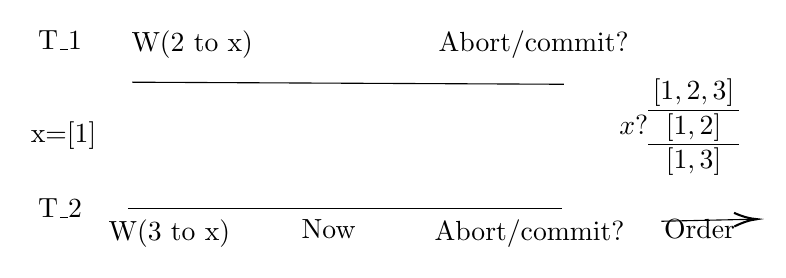
\begin{tikzpicture}[x=0.75pt,y=0.75pt,yscale=-1,xscale=1]
%uncomment if require: \path (0,300); %set diagram left start at 0, and has height of 300

%Straight Lines [id:da9500410641573396] 
\draw    (62.56,29) -- (270.56,30) ;
%Straight Lines [id:da7796185686481738] 
\draw    (60.56,90) -- (269.56,90) ;
%Straight Lines [id:da7329480179958066] 
\draw    (317.56,96) -- (361.56,95.04) ;
\draw [shift={(363.56,95)}, rotate = 178.75] [color={rgb, 255:red, 0; green, 0; blue, 0 }  ][line width=0.75]    (10.93,-3.29) .. controls (6.95,-1.4) and (3.31,-0.3) .. (0,0) .. controls (3.31,0.3) and (6.95,1.4) .. (10.93,3.29)   ;

% Text Node
\draw (16,3) node [anchor=north west][inner sep=0.75pt]   [align=left] {T\_1};
% Text Node
\draw (16,84) node [anchor=north west][inner sep=0.75pt]   [align=left] {T\_2};
% Text Node
\draw (61,3) node [anchor=north west][inner sep=0.75pt]   [align=left] {W(2 to x)};
% Text Node
\draw (50,94) node [anchor=north west][inner sep=0.75pt]   [align=left] {W(3 to x)};
% Text Node
\draw (209,3) node [anchor=north west][inner sep=0.75pt]   [align=left] {Abort/commit?};
% Text Node
\draw (207,94) node [anchor=north west][inner sep=0.75pt]   [align=left] {Abort/commit?};
% Text Node
\draw (317.56,94) node [anchor=north west][inner sep=0.75pt]   [align=left] {Order};
% Text Node
\draw (143,94) node [anchor=north west][inner sep=0.75pt]   [align=left] {Now};
% Text Node
\draw (12.5,47) node [anchor=north west][inner sep=0.75pt]   [align=left] {x=[1]};
% Text Node
\draw (296,25) node [anchor=north west][inner sep=0.75pt]   [align=left] {$x? \begin{array}{@{\,}c@{\,}}    [1,2,3]\\    \hline    [1,2]\\    \hline    [1,3]  \end{array} $};
\end{tikzpicture}
\vspace{2mm}

\subsection{P1 - Dirty Read}
The Dirty Read phenomena occur when a transaction T2 Reads an object that a concurrent transaction T1 has modified prior to T1 committing or aborting. This results in t2 returning an object that might never have existed in the transaction history. The preventative interpretation for P1 uses the same locking of the history via long-term and short-term locks as P0, such that P1 requires T1 to acquire a long write-lock and T2 to acquire (at least) a short-term read-lock.

\subsubsection{Example of violation}

Suppose transaction T1 modifies a x by appending [2]. Transaction T2 then reads that x before T1 performs a COMMIT. If T1 then performs a ROLLBACK, T2 will have read x = [1,2] a object that was never committed and that may thus be considered to have never existed.\\
\vspace{2mm}
\begin{figure}[h!]
\tikzset{every picture/.style={line width=0.75pt}} %set default line width to 0.75pt        
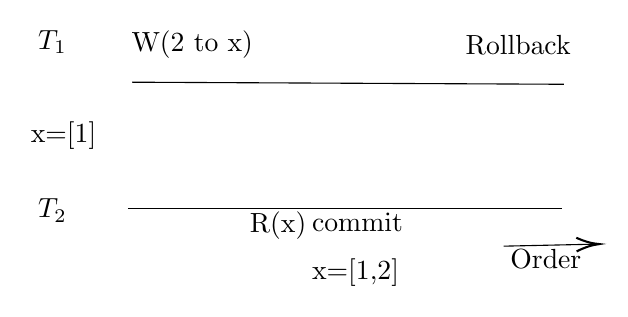
\begin{tikzpicture}[x=0.75pt,y=0.75pt,yscale=-1,xscale=1]
%uncomment if require: \path (0,300); %set diagram left start at 0, and has height of 300

%Straight Lines [id:da9500410641573396] 
\draw    (62.56,29) -- (270.56,30) ;
%Straight Lines [id:da7796185686481738] 
\draw    (60.56,90) -- (269.56,90) ;
%Straight Lines [id:da7329480179958066] 
\draw    (241.56,108) -- (285.56,107.04) ;
\draw [shift={(287.56,107)}, rotate = 178.75] [color={rgb, 255:red, 0; green, 0; blue, 0 }  ][line width=0.75]    (10.93,-3.29) .. controls (6.95,-1.4) and (3.31,-0.3) .. (0,0) .. controls (3.31,0.3) and (6.95,1.4) .. (10.93,3.29)   ;

% Text Node
\draw (16,3) node [anchor=north west][inner sep=0.75pt]   [align=left] {$T_1$};
% Text Node
\draw (16,84) node [anchor=north west][inner sep=0.75pt]   [align=left] {$T_2$};
% Text Node
\draw (61,3) node [anchor=north west][inner sep=0.75pt]   [align=left] {W(2 to x)};
% Text Node
\draw (118,90) node [anchor=north west][inner sep=0.75pt]   [align=left] {R(x)};
% Text Node
\draw (222,5) node [anchor=north west][inner sep=0.75pt]   [align=left] {Rollback};
% Text Node
\draw (148,91) node [anchor=north west][inner sep=0.75pt]   [align=left] {commit};
% Text Node
\draw (243.56,108) node [anchor=north west][inner sep=0.75pt]   [align=left] {Order};
% Text Node
\draw (12.5,47) node [anchor=north west][inner sep=0.75pt]   [align=left] {x=[1]};
% Text Node
\draw (148,113) node [anchor=north west][inner sep=0.75pt]   [align=left] {x=[1,2]};

\end{tikzpicture}
\caption{P1: Dirty Read between $T_1$ and $T_2$}
\end{figure}
\vspace{2mm}
\newpage
\subsection{P2 - Non-repeatable/Fuzzy Read}
The P2 violation occurs when a given transaction T1 reads the same object multiple times. A given transaction T2 modifies this object in-between any of these reads, causing T1 to see different versions of an object in the same transaction without modifying it. The preventative implementation for P2 requires the use of long read and write-locks; 

\subsubsection{Example of violation}
Suppose transaction T1 reads x as [1], transaction T2 then modifies x by appending 2 and commits. T1 then reads x as [1, 2].\\
\vspace{2mm}
\tikzset{every picture/.style={line width=0.75pt}} %set default line width to 0.75pt        
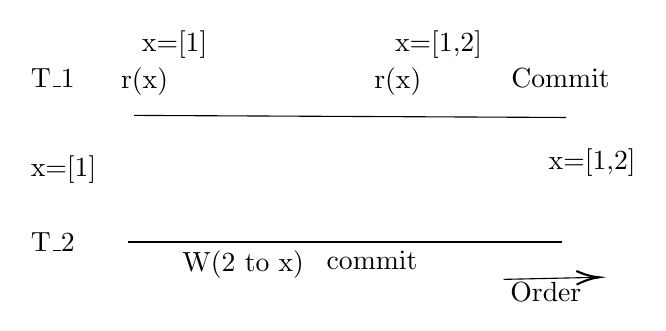
\begin{tikzpicture}[x=0.75pt,y=0.75pt,yscale=-1,xscale=1]
%uncomment if require: \path (0,300); %set diagram left start at 0, and has height of 300

%Straight Lines [id:da9500410641573396] 
\draw    (63.56,64) -- (271.56,65) ;
%Straight Lines [id:da7796185686481738] 
\draw    (60.56,125) -- (269.56,125) ;
%Straight Lines [id:da7329480179958066] 
\draw    (241.56,143) -- (285.56,142.04) ;
\draw [shift={(287.56,142)}, rotate = 178.75] [color={rgb, 255:red, 0; green, 0; blue, 0 }  ][line width=0.75]    (10.93,-3.29) .. controls (6.95,-1.4) and (3.31,-0.3) .. (0,0) .. controls (3.31,0.3) and (6.95,1.4) .. (10.93,3.29)   ;

% Text Node
\draw (12.5,40) node [anchor=north west][inner sep=0.75pt]   [align=left] {T\_1};
% Text Node
\draw (12.5,119) node [anchor=north west][inner sep=0.75pt]   [align=left] {T\_2};
% Text Node
\draw (85.56,128) node [anchor=north west][inner sep=0.75pt]   [align=left] {W(2 to x)};
% Text Node
\draw (56,40) node [anchor=north west][inner sep=0.75pt]   [align=left] {r(x)};
% Text Node
\draw (244,40) node [anchor=north west][inner sep=0.75pt]   [align=left] {Commit};
% Text Node
\draw (155,128) node [anchor=north west][inner sep=0.75pt]   [align=left] {commit};
% Text Node
\draw (243.56,143) node [anchor=north west][inner sep=0.75pt]   [align=left] {Order};
% Text Node
\draw (12.5,82) node [anchor=north west][inner sep=0.75pt]   [align=left] {x=[1]};
% Text Node
\draw (66,22) node [anchor=north west][inner sep=0.75pt]   [align=left] {x=[1]};
% Text Node
\draw (178,40) node [anchor=north west][inner sep=0.75pt]   [align=left] {r(x)};
% Text Node
\draw (188,22) node [anchor=north west][inner sep=0.75pt]   [align=left] {x=[1,2]};
% Text Node
\draw (262,79) node [anchor=north west][inner sep=0.75pt]   [align=left] {x=[1,2]};


\end{tikzpicture}
\vspace{2mm}
 


\subsection{P3 - Phantom Read}

The Phantom Read violation occurs when Transaction T1 performs a conditional read operation. Following this initial read, a second transaction T2 either inserts or modifies objects such that they meet the conditional requirement of T1, T2 then commits this change. T1 then performs the same conditional read operation containing additional objects. It is called Phantom Read because the new records seem to be of phantom origin. the preventative interpretation of P3 requires the acquisition of long-term Phantom read-locks

\subsubsection{Example of violation}

Suppose Transaction T1 selects all values >= 2, Transaction T2 then writes 3 to key x and commits. T1 then selects all values >= 2. the object x now matches this predicate and is included in the read operation. \\
\vspace{2mm}
\begin{figure}[h!]
\tikzset{every picture/.style={line width=0.75pt}} %set default line width to 0.75pt        
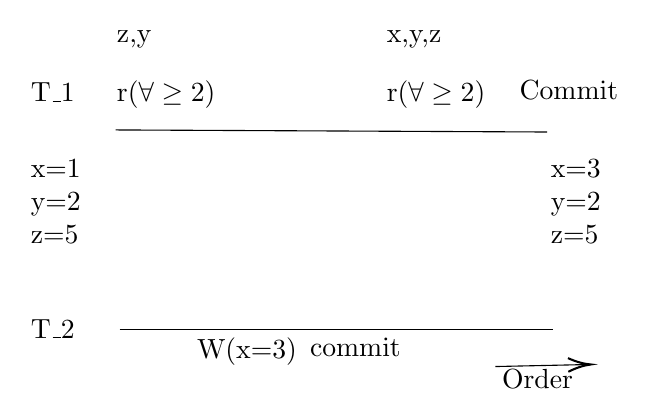
\begin{tikzpicture}[x=0.75pt,y=0.75pt,yscale=-1,xscale=1]
%uncomment if require: \path (0,300); %set diagram left start at 0, and has height of 300

%Straight Lines [id:da9500410641573396] 
\draw    (63.56,64) -- (271.56,65) ;
%Straight Lines [id:da7796185686481738] 
\draw    (65.56,160) -- (274.56,160) ;
%Straight Lines [id:da7329480179958066] 
\draw    (246.56,178) -- (290.56,177.04) ;
\draw [shift={(292.56,177)}, rotate = 178.75] [color={rgb, 255:red, 0; green, 0; blue, 0 }  ][line width=0.75]    (10.93,-3.29) .. controls (6.95,-1.4) and (3.31,-0.3) .. (0,0) .. controls (3.31,0.3) and (6.95,1.4) .. (10.93,3.29)   ;

% Text Node
\draw (21.5,40) node [anchor=north west][inner sep=0.75pt]   [align=left] {T\_1};
% Text Node
\draw (21.5,154) node [anchor=north west][inner sep=0.75pt]   [align=left] {T\_2};
% Text Node
\draw (101.56,163) node [anchor=north west][inner sep=0.75pt]   [align=left] {W(x=3)};
% Text Node
\draw (63,39) node [anchor=north west][inner sep=0.75pt]   [align=left] {r($\forall \geq 2$)};
% Text Node
\draw (257,39) node [anchor=north west][inner sep=0.75pt]   [align=left] {Commit};
% Text Node
\draw (156,163) node [anchor=north west][inner sep=0.75pt]   [align=left] {commit};
% Text Node
\draw (248.56,178) node [anchor=north west][inner sep=0.75pt]   [align=left] {Order};
% Text Node
\draw (21.5,77) node [anchor=north west][inner sep=0.75pt]   [align=left] {x=1\\y=2\\z=5};
% Text Node
\draw (193,15) node [anchor=north west][inner sep=0.75pt]   [align=left] {x,y,z};
% Text Node
\draw (63,15) node [anchor=north west][inner sep=0.75pt]   [align=left] {z,y};
% Text Node
\draw (193,39) node [anchor=north west][inner sep=0.75pt]   [align=left] {r($\forall \geq 2$)};
% Text Node
\draw (272,77) node [anchor=north west][inner sep=0.75pt]   [align=left] {x=3\\y=2\\z=5};

\end{tikzpicture}
\caption{P3: Phantom Read $T_1$ and $T_2$}
\end{figure}
\vspace{2mm}
\newpage
\subsection{Currently Described Anomalies} \todo[author=Mark]{ Unsure what to name this.}

Following the ANSI standard and Adya et al. \cite{Adya99weakconsistency} a significant amount of discoveries have been made that describe anomalies not accounted for in most definitions of consistency models. A recent paper by Haixiang Li et al. \cite{li2021coo} describes a total of 18 anomalies either described in standards or paper in the past 30 years; The paper mentions that all these definitions are defined case by case and not in a rigors mathematically manner. The paper includes the following sentence: 
\begin{quote}
    "Definition of data anomalies. Although there are so many data anomalies, but it seems that data anomalies are not explicitly defined. There is no universally accepted definition of data anomalies in academia and industry, and the understanding of data anomalies is only in the way of case-by-case" \cite{li2021coo}
\end{quote}

The 18 transactional anomalies are listed below. These definitions will not be explored deeper unless relevant for the thesis.

\vspace{2mm}

\begin{table}[h]
    \begin{tabular}{l|l|l}
        No & Anomaly, reference, year                        & Formal definition  \\ \hline
        1  & Dirty Write {[}1{]} 1992                        & $W_1 [x_1 ]...W_2 [x_2 ]...((C_1 or A_1) and (C_2 or A_2) in any order) $  \\
        2  & Lost Update {[}6{]} 1995                        & $  R_1 [x_0 ]...W_2 [x_1 ]...C_2...W_1 [x_2 ] $ \\
        3  & Dirty Read {[}1{]} 1992                         & $ W_1 [x ]...R_2 [x ]...(A_1 and C_2 in either order) $ \\
        4  & Aborted Reads {[}45{]} 2015, {[}2{]} 2000       & $ W_1 [x : i]...R_2 [x : i]...(A_1 and C_2 in any order) $  \\
        5  & Fuzzy/Non-repeatable Read {[}1{]} 1992          & $ R_1 [x ]...W_2 [x ]...C_2...R_1 [x ]...C_1 $  \\
        6  & Phantom {[}1{]} 1992                            & $ R_1 [P ]...W_2[y in P]...C_2...R_1 [P ]...C_1 $  \\
        7  & Intermediate Reads {[}45{]} 2015, {[}2{]} 2000  & $ W_1 [x : i]...R_2 [x : i]...W_1 [x : j]...C_2  $  \\
        8  & Read Skew {[}6{]} 1995                          & $ R_1 [x_0 ]...W_2 [x_1 ]...W_2 [y_1 ]...C_2...R_1 [y_1] $ \\
        9  & Unnamed Anomaly {[}38{]} 2000                   & \begin{tabular}[c]{@{}l@{}}$ R_1 [y]...R_2 [x ]...W_2 [x ]...R_2 [y]...W_2 [y]...C_2...R_3 [x ]...W_3 [x ]$\\$...R_3 [z]...W_3 [z]...C_3...R_1 [z]...C_1 $\end{tabular}      \\
        10 & Fractured Reads {[}16{]} 2017, {[}5{]} 2014     & $ R_1 [x_0]...W_2 [x_1 ]...W_2 [y_1 ]...C_2...R_1 [y_1 ] $ \\
        11 & Serial-Concurrent-phenomenon {[}12{]} 2014      & $ R_1 [x_0 ]...W_2 [x_1 ]...W_2 [y_1 ]...C_2...R_1 [y_1 ] $  \\
        12 & Cross-phenomenon {[}12{]} 2014                  & $ R_1 [x_0 ]...R_2 [y_0 ]...W_3 [x_1 ]...C_3...W_4 [y_1 ]...C_4...R_2 [x_1 ]...R_1 [y_1 ] $ \\
        13 & Long Fork Anomaly {[}16{]} 2017                 & $ R_1 [x_0 ]...R_2 [y_0 ]...W_3 [x_1 ]...C_3...W_4 [y_1 ]...C_4...R_2 [x_1 ]...R_1 [y_1 ] $ \\
        14 & Causality Violation Anomaly {[}16{]} 2017       & $ R_1 [x_0 ]...W_2 [x_1 ]...C_2...R_3 [x_1 ]...W_3 [y_1 ]...C_3...R_1 [y_1 ] $  \\
        15 & Read-only Transaction Anomaly {[}26, 43{]} 2004 & \begin{tabular}[c]{@{}l@{}}$ R_1 [x_0, 0]...R_1 [y_0, 0]...R_2 [y_0, 0]...W_2 [y_1, 20]...C_2$\\$...R_3 [x_0,0]...R_3 [y_1, 20]...C_3...W_1 [x_2, -11]...C_1 $\end{tabular} \\
        16 & Write Skew {[}6{]} 1995                         & $ R_1 [x_0 ]...R_2 [y_0 ]...W_1 [y_1 ]...W_2 [x_1 ] $   \\
        17 & Predicate-based Write Skew {[}27{]} 2005        & $ R_1 [P ]...R_2 [P ]...W_1 [y_1 in P]...W_2[x_1 in P] $  \\
        18 & Read Partial-Committed {[}44{]} 2019            & $ R_1[x] W_2[x] W_2[y] C_2 R_1[Y] C_1 $ 
    \end{tabular}
    \caption{Transaction anomalies from the COO paper}
\end{table}


\vspace{2mm}

Outside of the above paper, other anomalies and issues exist within databases, a deeper investigation into these will not take place, but a short explanation will be given here for issues that often occur to create awareness about the issue,
\begin{itemize}
    \item Split Brain, A Split Brain occurs when a distributed database is partitioned into two or more fragments that cannot reach each other. However, both remain active with two leaders and continue to process transactions, leading to each fragment believing in separate histories. Split Brain is a regular occurrence in distributed databases.\cite{aphyrelasticsearch, jepsenscylla, jepsenhazelcast}, Some systems can recover from this but often lose data during the healing process.
    \item Poor handling of quorum
\end{itemize}

\newpage
\section{Consistency models}

\begin{wrapfigure}{r}{0.5\linewidth}
    \centering
    \includegraphics[scale=0.4]{images/consistency models.PNG}
    \caption{Picture from jepsen.io/consistency}
    \label{fig:jepsenioconsistency}
\end{wrapfigure}
For explaining the concepts within consistency, we will use a paper by Ballis et al. on "Highly available transactions"\cite{HighlyAvailableTransactionsVirtuesandLimitations} that contains a good model for presenting the different consistency models and their relation to other consistency models. A focus will be on Transactional models, so not all of the BASE models are covered.\\

\subsection{Strict Serializability}

For a system to have Strict Serializability, it is required that the entire system operationally appears to occur in order regarding both the order and the real-time of the operations. Within the CAP theorem, this would be considered a CA system.\\
\vspace{5mm}
Formally Strict Serializability is defined as a Serviceable system compatible with a Time-dependent order.
"A history is serializable if it is equivalent to one in which transactions appear to execute sequentially, i.e., without interleaving. A (partial) precedence order can be defined on non-overlapping pairs of transactions in an obvious way. A history is strictly serializable if the transactions' order in the sequential history is compatible with their precedence order." \cite{Herlihy1990Linearizability}\\
\vspace{5mm}
Here it should be clarified what is meant by "the obvious way." For transactions A and B, A proceeds B if A completes prior to transaction B starting. Essentially a Serializable system with the time constraint from Linearizability.

SS cannot be totally or sticky available in the event of a network partition. In this case, some or all nodes will be stuck; this is due to the nature of the Strict Serializable consistency model, where transactions operate on the system as a whole, as in the case of a partition in the distributed system, this is impossible. There can be cases where replicate nodes are partitioned from the primary nodes, and the primary nodes can continue with some degradation but where the replicas either shut down or serve stale data. In the case of primary nodes partitioning, the system would be unable to resume due to not being able to commit a given transaction to the entire system.


\vspace{2mm}
\begin{table}[h!]
    \begin{tabular}{l|l|l|l}
        $T_1$            & $T_2$            & $T_3$   & $T_4$   \\
        $W(x_1)$ &      &      &      \\
        $R(y_0)$ &      &      &      \\
        C    &      &      &      \\
        & $R(x_1)$ &      &      \\
        & $R(y_0)$ &      &      \\
        & C    &      &      \\
        &      & $R(z_0)$ &      \\
        &      & $W(h_1)$ &      \\
        &      & C    &      \\
        &      &      & $R(x_1)$ \\
        &      &      & C
    \end{tabular}
    \caption{Transactions are ordered chronological in time, and executed as such.}
\end{table}

\vspace{2mm}


\subsection{Serializable}

Serializability is a relaxation of the Strict Serializability consistency model that foregoes that real-time constraint. It defines systems where transactions occur in some total order. It is formally defined in the ANSI SQL 1999 spec as follows.

\begin{quote}
"The execution of concurrent SQL-transactions at isolation level SERIALIZABLE is guaranteed to be serializable. A serializable execution is defined to be an execution of the operations of concurrently executing SQL-transactions that produces the same effect as some serial execution of those same SQL-transactions. A serial execution is one in which each SQL-transaction executes to completion before the next SQL-transaction begins."\cite{ansisql1999}\\
\end{quote}
\vspace{5mm}

The above implies that Serializability of the transactions does not only apply to the objects in use but the system as a whole. This means that in the case of a network partition, some or all notes will be stuck until the network is healed. Further, we can observe stale reads as no real-time constraint is enforced. This occurs when process A completes a write, then process B begins a read, and the read is not guaranteed to observe the write from process A.
\\ \vspace{5mm}

Serializable has a further limitation due to having no real-time constraint; SR allows pathological orderings. This allows a serializable database to discard, write, and increment operations that are never observed by executing them at the very end of the history. Furthermore, read operations can always return an empty state by placing the transaction at the beginning of the history. However, it should be noted that most implementation does not take advantage of this.
\\ \vspace{5mm}
SR follows closely to S-SR regarding partition tolerance and availability and is therefore considered a CA database.
\\ \vspace{5mm}
\vspace{2mm}
\begin{table}[h]
    \begin{tabular}{l|l|l|l}
        T1   & T2   & T3   & T4   \\
        w(z) &      &      &      \\
        & r(z) &      &      \\
        &      &      & r(z) \\
        & w(y) &      &      \\
        &      &      & c    \\
        &      & r(y) &      \\
        & c    &      &      \\
        &      & w(h) &      \\
        r(x) &      &      &      \\
        c    &      &      &      \\
        &      & c    &
    \end{tabular}
    \caption{Transactions are ordered chronological in time and executed in a way that makes it possible for the operations to occur atomically such that they appear to have been executed in order transaction-wise. }
\end{table}
\vspace{2mm}



\newpage
\subsection{Repeatable Read}

Repeatable Read (RR) closely resembles the Serializable consistency model, however in RR, we allow phantoms. This implies that if T1 reads a predicate like "select all from alarms with the newest timestamp," another transaction T2 is able to create or modify values within the predicate before T1 commits. So if the transaction T1 performs the read again, this predicate might not be stable.
\\ \vspace{5mm}
RR contains the above relaxation; however, this relaxation implies more than meets the eye. For example, repeatable read does not guarantee repeatable reads in the sense that we might consider. This is due to RR not requiring any real-time constraint; this allows for a situation where process A performs a write, and after process A completes process B performs a read. However, this read is not guaranteed to obverse the write from process A. Furthermore, as no per-process ordering of transactions is required, process A can write something and then fail to observe that write in a subsequent transaction.
\\ \vspace{5mm}
It should also be noted that RR allows for the same pathological ordering of operations as a Serializable database.
\vspace{2mm}
\begin{table}[h]
    \begin{tabular}{l|l|l|l}
        T1            & T2            & T3   & T4   \\
        &               &      & r(y) \\
        &               &      & c    \\
        w(p$_1$ to y) &               &      &      \\
        r(p in y)     &               &      &      \\
        &               &      &      \\
        & w(p$_2$ to y) &      &      \\
        & c             &      &      \\
        r(p in y)     &               &      &      \\
        w(z)          &               &      &      \\
        c             &               &      &      \\
        &               & r(z) &      \\
        &               & w(x) &      \\
        &               & c    &
    \end{tabular}
    \caption{T1 shows an example of a valid transaction with a phantom, and T4 could be placed at the beginning of the history, returning the "empty" result. Both are valid transactions within RR.}
\end{table}
\vspace{2mm}

\newpage
\subsection{Cursor Stability}
Cursor Stability closely resembles repeatable read where RR locks the objects until committed. Cursor Stability locks the objects until the cursor moves on or until committed. This allows for different behavior depending on implementation but is formally defined by which phenomena it allows and which it prohibits. \cite{Adya99weakconsistency}\\
\begin{itemize}
    \item G-cursor(x): the directed serialization graph, restricted to a single object x, contains an anti-dependency cycle and at least one write-dependency edge.
    \item g1:
    \begin{enumerate}
        \item G1a (Aborted Reads): A transaction observes an object (perhaps via a predicate) modified by an aborted transaction. Intuitively, transactions have to commit for us to read them.
        \item G1b (Intermediate Reads): A transaction observes an object (perhaps via a predicate) modified by a transaction that was not that transaction's final modification of that object. Intuitively, transactions have to finish before we can read them,
        \item G1c (Circular Information Flow): the Directed Serialization Graph of transactions contains a directed cycle consisting entirely of dependency edges. Intuitively, if transaction T1 is affected by T2, T2 cannot be affected by T1.
    \end{enumerate}
\end{itemize}
Furthermore, since cursor stability is strictly stronger than read committed, it also prohibits the ANSI phenomena:
\begin{itemize}
    \item P0 (Dirty Write): w1(x) … w2(x)
    \item P1 (Dirty Read): w1(x) … r2(x)
\end{itemize}

but allows:
\begin{itemize}
    \item P2 (Fuzzy Read): r1(x) … w2(x)
    \item P3 (Phantom): r1(P) … w2(y in P)
\end{itemize}


\todo[author=Mark]{Make diagram Cursor Stability}
\newpage
\subsection{Snapshot Isolation}

Snapshot Isolation behaves differently to any of the systems. It can be considered more as a \textbf{try: commit() catch: abort()} . We perform our transaction in an independent branch and commit/merge to the database on commit; if there are any conflicts with an already committed transaction, the transaction is simply aborted.
\\ \vspace{5mm}
Snapshot Isolation, like Readable Read, operates on an object level and allows for the same behavior. Items are stable once read; however, the predicate again isn't. We can fail to observe a previously committed transaction and place operations in arbitrary places in the transaction due to no Linearizability constraint. It also allows sub-operations to interleave. This can result in write skews, which allow transactions to read overlapping states, modify disjoint sets of objects, then commit; and a read-only transaction anomaly involving partially disjointing write sets.
\\ \vspace{5mm}

It should also be noted that there exist multiple versions of Snapshot Isolation, one being prefix-consistent snapshot isolation that enforces process-level transaction ordering, which prevents a given process from failing to observe a previous transaction; and another being parallel snapshot isolation that allows for total availability but this allows for long fork anomalies, as each node has its own transaction ordering.
\\ \vspace{5mm}
Formally Snapshot Isolation is defined by Berenson et al.\cite{Berensonetal}. as:

\begin{displayquote}
… each transaction reads data from a snapshot of the (committed) data as of the time the transaction started, called its Start-Timestamp. This time may be any time before the transaction's first Read. A transaction running in Snapshot Isolation is never blocked attempting a read as long as the snapshot data from its Start-Timestamp can be maintained. The transaction's writes (updates, inserts, and deletes) will also be reflected in this snapshot, to be read again if the transaction accesses (i.e., reads or updates) the data a second time. Updates by other transactions active after the transaction Start-Timestamp are invisible to the transaction.
\\
When the transaction T1 is ready to commit, it gets a Commit-Timestamp, larger than any existing Start-Timestamp or Commit-Timestamp. The transaction successfully commits only if no other transaction T2 with a Commit-Timestamp in T1's execution interval [StartTimestamp, Commit-Timestamp] wrote data that T1 also wrote. Otherwise, T1 will abort. This feature, called First-committer-wins prevents lost updates (phenomenon P4). When T1 commits, its changes become visible to all transactions whose Start-Timestamps are larger than T1's Commit-Timestamp.
\end{displayquote}

There also exist multiple other definitions from Cerone et al. \cite{CeroneBernardiGotsman} and Crooks et al. \cite{CrooksPuAlvisiClement}

\vspace{2mm}
\begin{table}[h!]
    \begin{tabular}{l|l|l|l}
        $T_1$            & $T_2$            & $T_3$   & $T_4$   \\
        &      &      & $R(y_0)$ \\
        &      &      & C    \\
        $W(y_1)$ &      &      &      \\
        $R(y_1)$ &      &      &      \\
        &      &      &      \\
        & $W(y_2)$ &      &      \\
        &      &      &      \\
        $R(y_1)$ &      &      &      \\
        $W(z_1)$ &      &      &      \\
        C    &      &      &      \\
        & a    & $R(z_1)$ &      \\
        &      & $W(x_1)$ &      \\
        &      & C    &
    \end{tabular}
    \caption{$T_1$ and $T_2$ contains a conflict that causes $T_2$ to abort as $T_1$ commits prior to $T_2$}
\end{table}
\vspace{2mm}

\newpage
\subsection{Monotonic Atomic View}
The Monotonic Atomic view(MAV) model is a relaxation of snapshot isolation. It requires that effects by transactions are fully visible once read by other transactions, such that T1 may perform w(1), w(2), w(2), c. These three sub-operations effects should all either be fully visible or not at all, so partial transactions are not allowed. Formally this is defined by Bailis et al. \cite{HighlyAvailableTransactionsVirtuesandLimitations}
\begin{quote}
    "Under MAV, once some of the effects of a transaction Ti are observed by another transaction Tj, thereafter, all effects of Ti are observed by Tj. That is if a transaction Tj reads a version of an object that transaction Ti wrote, then a later read by Tj cannot return a value whose later version is installed by Ti."
\end{quote}


Furthermore, by Adya et al. \cite{Adya99weakconsistency} as prohibiting:
\begin{itemize}
    \item G1b (Intermediate Reads): A transaction observes an object (perhaps via a predicate) modified by a transaction that was not that transaction's final modification of that object. Intuitively, transactions have to finish before we can read them,
\end{itemize}

Further, since MAV is strictly stronger than Read Committed, it also disallows the ANSI phenomena Dirty Write(P0), Dirty Read (P1) but allows Fuzzy Read (P2) and Phantom (P3)

\subsection{Read Committed}
The Read Committed transaction model is the first non-atomic transaction model where partial visibility of committed transactions is permitted. This however, might lead to foreign key constraint issues, among other problems where required data joins are performed due to not yet visible values.
\\ \vspace{5mm}

Formally it is defined in ANSISQL1999\cite{ansisql1999} by disallowing P1 ("Dirty read" ). In the Microsoft paper, Berenson et al. \cite{Berensonetal} it is observed that the ANSI specification allows multiple interpretations, one of which allows non-serializable histories. Here Adya et al.\cite{Adya99weakconsistency} is commonly used as it provides a concrete specification based on the unambiguous ANSI specification.
\\ \vspace{5mm}

\todo[author=Mark]{TODO Make Diagram Read committed}

\subsection{Read Uncommitted}
Read Uncommitted as defined by ANSI allows all behavior. However, this has been challenged by Berenson et al. \cite{Berensonetal} where they argue that Read Uncommitted should disallow dirty writes. This is also the non-ANSI defacto definition as per Adya et al. \cite{Adya99weakconsistency} which again provides a better definition based on what can be interpreted from the loose definition in ANSISQL99\cite{ansisql1999}. It should be noted that due to the loose specification in ANSI, multiple mainstream interpretations exist.\\

by the Aday's specification Read Uncommitted disallows
\begin{itemize}
    \item Dirty Write(P0)
\end{itemize}
But allows
\begin{itemize}
    \item Dirty read(P1)
    \item Fuzzy Read (P2)
    \item Phantom (P3)
\end{itemize}

\subsection{Non-transaction models (BASE)}
The category of BASE transaction models is not considering the order of transactions but rather the ordering of operations in real-time. Only Linearizable and Sequential Consistency are introduced here. Other BASE models exist. The core ones are Casual Consistency, Writes Follows Reads, Monotonic Reads, Monotonic Writes, and Read Your Writes.

\subsubsection{Linearizable}
Linearizability is the strongest single object consistency model that requires operations to occur in an order consistent with real-time, and the operations themselves should occur atomically. It should also be noted that Linearizability is not tolerant to network partitions and should be considered a CA model according to the CAP theorem.

it is formalized  in \cite{Linearizability} and later specified  in \cite{ConsistencyinNonTransactionalDistributedStorageSystems} where it's defined by 3 requirements

\begin{itemize}
    \item Single Order (there exists some total order of operations)
    \item RealTime (consistent with the real time bound)
    \item RVal (obeying the single-threaded laws of the associated object's datatype)
\end{itemize}

\subsubsection{Sequential Consistency}
Sequential Consistency (SC) is a relaxation of Linearizability. Unlike Linearizability, SC is a concurrent model. The requirement is that all operations follow a total order, which is consistent across all processes. However, since a Total order is required, the model cannot tolerate partitions, and some or all nodes will be unable to make progress. 
\\ \vspace{5mm}
One of the phenomena SC allows is Stale Reads. All processes have to follow the same total order, but there is not a strong constraint concerning how far a process may be behind or ahead, and it may return an arbitrarily stale state. However, once a given node A observes some operations from a separate node B, A may never observe a state prior to B.

Formally SC was defined by Leslie Lamport\cite{Lamport1979how}, however Viotti and Vukolić\cite{ConsistencyinNonTransactionalDistributedStorageSystems} formalized it into three requirements:
\begin{itemize}
    \item SingleOrder (there exists some total order of operations)
    \item PRAM (the session order (the order of operations on each process) is a subset of the visibility order (what operations are visible to a given operation).)
    \item RVal (the order must be consistent with the semantics of the datatype)
\end{itemize}

\todo[author=Mark]{Two of the consistency models were already mentioned in the previous section namely Atomic Consistency and Sequential Consistency. There exist two more models within common use, which are Causal Consistency and Eventual Consistency. They differ in the way the consistency is handled by all end up in the same state eventually.}



\section{Directed Serialization graphs}

Directed Serialization graphs(DSG) are to reason about a history of Transactions and operations within a transaction. Each node represents a committed transaction, and edges represent different types of direct conflicts. \\ using these conflicts, we can reason about what order transactions were executed in and if any transactional phenomena of anomalies occurred. These are defined in terms of DSG cycles and conflict relations. 
\subsection{Transaction conflicts relations}
\subsubsection{Read-dependency}

The Read-dependency is when a Transaction $T_j$ directly depends on a write from a transaction $T_i$ where $T_i$ writes some object $x_i$ and $T_j$ reads $x_i$. This relation is also called Write-Read (wr), as one transaction writes an object and a second transaction depends on this prior write.
        
\vspace{2mm}
\vspace{2mm}
\tikzset{every picture/.style={line width=0.75pt}} %set default line width to 0.75pt        

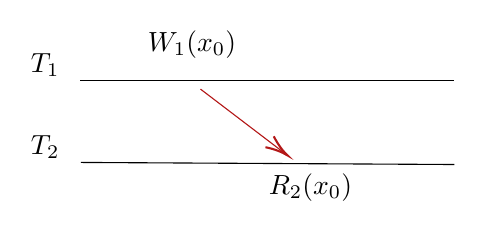
\begin{tikzpicture}[x=0.75pt,y=0.75pt,yscale=-1,xscale=1]
%uncomment if require: \path (0,300); %set diagram left start at 0, and has height of 300

%Straight Lines [id:da9351620672631715] 
\draw    (70.33,79.67) -- (250.33,79.67) ;
%Straight Lines [id:da20316716985592453] 
\draw    (70.67,119.33) -- (250.67,120.33) ;
%Straight Lines [id:da3663864520178606] 
\draw [color={rgb, 255:red, 179; green, 23; blue, 23 }  ,draw opacity=1 ]   (128.33,84) -- (168.74,114.79) ;
\draw [shift={(170.33,116)}, rotate = 217.3] [color={rgb, 255:red, 179; green, 23; blue, 23 }  ,draw opacity=1 ][line width=0.75]    (10.93,-3.29) .. controls (6.95,-1.4) and (3.31,-0.3) .. (0,0) .. controls (3.31,0.3) and (6.95,1.4) .. (10.93,3.29)   ;

% Text Node
\draw (45.33,65.67) node [anchor=north west][inner sep=0.75pt]   [align=left] {$T_1$};
% Text Node
\draw (45.33,105) node [anchor=north west][inner sep=0.75pt]   [align=left] {$T_2$};
% Text Node
\draw (101.67,54.67) node [anchor=north west][inner sep=0.75pt]   [align=left] {$W_1(x_0)$};
% Text Node
\draw (160,123.67) node [anchor=north west][inner sep=0.75pt]   [align=left] {$R_2(x_0)$};

\end{tikzpicture}
\vspace{2mm}
\vspace{2mm}

We have a history H. as follows.
\begin{equation}
    History\ H: [T_1(W(x_0)), T_2(R(x_0))]
\end{equation}

This history contains two transactions $T_i$ followed by $T_j$. $T_i$ writes version $x_0$, which is later read by $T_j$, thus item-read-depends on $T_i$. this wr is also denoted by the red arrow in the above illustration.
    
A SQL example of this relation would be the below script
        
\begin{lstlisting}
update accounts set balance = 42 where id = 1;
select * from accounts where id = 1;
\end{lstlisting}
        
        
\subsubsection{predicate-based read dependency (wr)}
A Predicate read dependency occurs when a transaction $T_j$ performs an operation containing multiple reads while a concurrent $T_i$ performs writes within the predicate of $T_j$. This occurs if $T_i$ write $x_i$, $x_h$ precedes $x_i$ in the history, and $x_h$ matches Predicate where $x_i$ does not or opposite were $x_h$ does not match the predicate whereas $x_i$ does.\\

This case of WR dependency gives the symptom of objects appearing or disappearing within a transaction. 

\vspace{2mm}
\vspace{2mm}
\begin{figure}[h!]
\tikzset{every picture/.style={line width=0.75pt}} %set default line width to 0.75pt        

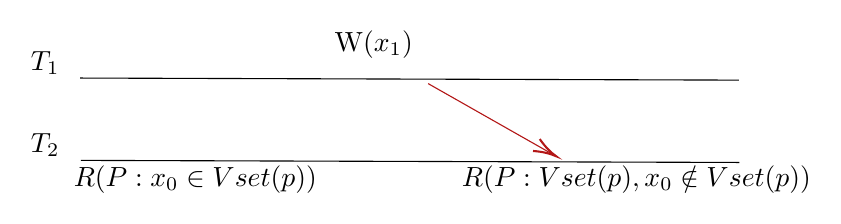
\begin{tikzpicture}[x=0.75pt,y=0.75pt,yscale=-1,xscale=1]
%uncomment if require: \path (0,300); %set diagram left start at 0, and has height of 300

%Straight Lines [id:da9351620672631715] 
\draw    (41.33,82) -- (358.67,83) ;
%Straight Lines [id:da20316716985592453] 
\draw    (41.67,121.67) -- (359,122.67) ;
%Straight Lines [id:da3663864520178606] 
\draw [color={rgb, 255:red, 179; green, 23; blue, 23 }  ,draw opacity=1 ]   (209,84.67) -- (268.93,118.68) ;
\draw [shift={(270.67,119.67)}, rotate = 209.58] [color={rgb, 255:red, 179; green, 23; blue, 23 }  ,draw opacity=1 ][line width=0.75]    (10.93,-3.29) .. controls (6.95,-1.4) and (3.31,-0.3) .. (0,0) .. controls (3.31,0.3) and (6.95,1.4) .. (10.93,3.29)   ;

% Text Node
\draw (16.33,68) node [anchor=north west][inner sep=0.75pt]   [align=left] {$T_1$};
% Text Node
\draw (16.33,107.33) node [anchor=north west][inner sep=0.75pt]   [align=left] {$T_2$};
% Text Node
\draw (162.67,58) node [anchor=north west][inner sep=0.75pt]   [align=left] {W($x_1$)};
% Text Node
\draw (224,123) node [anchor=north west][inner sep=0.75pt]   [align=left] {$R(P:Vset(p),x_0\notin Vset(p)$)};
% Text Node
\draw (37,123) node [anchor=north west][inner sep=0.75pt]   [align=left] {$R( P:x_0 \in Vset(p))$};


\end{tikzpicture}
\caption{predicate-based read dependency between $T_1$ and $T_2$, (wr)}
\end{figure}
\vspace{2mm}
\vspace{2mm}


Transaction $T_2$ sees $x_0$ in it's first predicate read, however in the second read nothing is observed as $x_0$ was overwritten by $x_1$ via $T_1$. \\

We have a history H. as follows.
\begin{equation}
    History\ H: [T_1(W(x_1)), T_2(R(x_0),R(\emptyset))]
\end{equation}

A SQL example of this relation would be the below script.

\begin{lstlisting}
select * from accounts where balance > 0;
update accounts set balance = -42 where id = 1;
select * from accounts where balance > 0;
\end{lstlisting}
        
        
\subsubsection{Write-dependency (ww)}
A write dependency occurs when transaction $T_j$ directly depends on $T_i$ if $T_i$ writes $x_i$, and $T_j$ writes the version of x following $T_i$ in the history. the relation is named ww as two writes to the same object with only one persisting.

\vspace{2mm}

\tikzset{every picture/.style={line width=0.75pt}} %set default line width to 0.75pt        

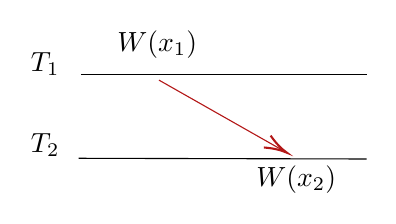
\begin{tikzpicture}[x=0.75pt,y=0.75pt,yscale=-1,xscale=1]
%uncomment if require: \path (0,300); %set diagram left start at 0, and has height of 300

%Straight Lines [id:da9351620672631715] 
\draw    (41.67,80) -- (179.67,80) ;
%Straight Lines [id:da20316716985592453] 
\draw    (40.67,120.33) -- (179.33,120.67) ;
%Straight Lines [id:da3663864520178606] 
\draw [color={rgb, 255:red, 179; green, 23; blue, 23 }  ,draw opacity=1 ]   (79.33,82.67) -- (139.26,116.68) ;
\draw [shift={(141,117.67)}, rotate = 209.58] [color={rgb, 255:red, 179; green, 23; blue, 23 }  ,draw opacity=1 ][line width=0.75]    (10.93,-3.29) .. controls (6.95,-1.4) and (3.31,-0.3) .. (0,0) .. controls (3.31,0.3) and (6.95,1.4) .. (10.93,3.29)   ;

% Text Node
\draw (16.33,68) node [anchor=north west][inner sep=0.75pt]   [align=left] {$T_1$};
% Text Node
\draw (16.33,107.33) node [anchor=north west][inner sep=0.75pt]   [align=left] {$T_2$};
% Text Node
\draw (58,57.67) node [anchor=north west][inner sep=0.75pt]   [align=left] {$W(x_1)$};
% Text Node
\draw (125,122.67) node [anchor=north west][inner sep=0.75pt]   [align=left] {$W(x_2)$};
\end{tikzpicture}
\vspace{2mm}


Transaction $T_2$ overwrites the object $x_1$ written by $T_1$ implying a Write-depends on $T_1$, The dependency is denoted by the red arrow in the graph. \\

\begin{equation}
    History\ H: [T_1(W(x_1)), T_2(W(x_2))]
\end{equation}

A SQL example of this relation would be the below script

\begin{lstlisting}
update accounts set balance = 42 where id = 42;
update accounts set balance = -42 where id = 42;
\end{lstlisting}


\subsubsection{Anti-dependency (rw)}
A read-write-dependency, formally known as an anti-dependency, occurs when a transaction overwrites a version observed by another transaction. i.e., transaction T1 reads an object x, x is then modified by transaction T2.

\vspace{2mm}
\vspace{2mm}
\begin{figure}[h!]

\tikzset{every picture/.style={line width=0.75pt}} %set default line width to 0.75pt        

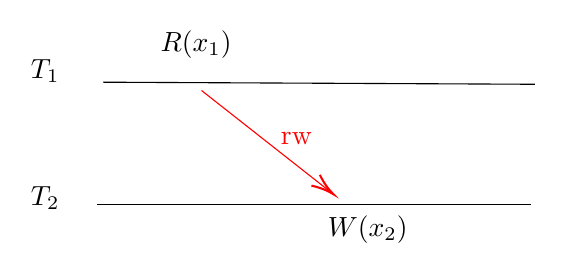
\begin{tikzpicture}[x=0.75pt,y=0.75pt,yscale=-1,xscale=1]
%uncomment if require: \path (0,300); %set diagram left start at 0, and has height of 300

%Straight Lines [id:da9500410641573396] 
\draw    (50.56,42) -- (258.56,43) ;
%Straight Lines [id:da7796185686481738] 
\draw    (47.56,101) -- (256.56,101) ;
%Straight Lines [id:da9563274467788809] 
\draw [color={rgb, 255:red, 255; green, 0; blue, 0 }  ,draw opacity=1 ]   (98,46) -- (159.99,94.76) ;
\draw [shift={(161.56,96)}, rotate = 218.19] [color={rgb, 255:red, 255; green, 0; blue, 0 }  ,draw opacity=1 ][line width=0.75]    (10.93,-3.29) .. controls (6.95,-1.4) and (3.31,-0.3) .. (0,0) .. controls (3.31,0.3) and (6.95,1.4) .. (10.93,3.29)   ;

% Text Node
\draw (14.5,30) node [anchor=north west][inner sep=0.75pt]   [align=left] {$T_1$};
% Text Node
\draw (14.5,91) node [anchor=north west][inner sep=0.75pt]   [align=left] {$T_2$};
% Text Node
\draw (157.56,105) node [anchor=north west][inner sep=0.75pt]   [align=left] {$W(x_2)$};
% Text Node
\draw (77,16) node [anchor=north west][inner sep=0.75pt]   [align=left] {$R(x_1)$};

\draw (135,65) node [anchor=north west][inner sep=0.75pt]  [color={rgb, 255:red, 255; green, 0; blue, 0 }  ,opacity=1 ] [align=left] {rw};

\end{tikzpicture}
    \caption{Anti-dependency between the read of $T_1$ and the write of $T_2$}
\end{figure}
\vspace{2mm}
\vspace{2mm}



Transaction $T_1$ reads $X_1$, this object is then modified by $T_2$ and therefor anti-depends on $T_1$, i,e $T_2$ occurred after $T_1$ in the history.
\begin{equation}
    History\ H: [T_1(r(x_0)), T_2(W(x_1))]
\end{equation}


A SQL example of this relation would be the below script:
\begin{lstlisting}
  select * from accounts where id = 42;
  update accounts set balance = 2022 where id = 42;
\end{lstlisting}

\subsection{phenomena defined via cycles and conflicts}

\subsection{G0: Dirty Writes}
A history exhibits phenomenon G0 if the DSG contains a directed cycle consisting entirely of write-dependency edges.

\vspace{2mm}
\tikzset{every picture/.style={line width=0.75pt}} %set default line width to 0.75pt        

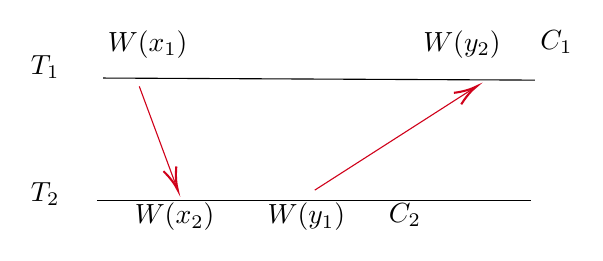
\begin{tikzpicture}[x=0.75pt,y=0.75pt,yscale=-1,xscale=1]
%uncomment if require: \path (0,300); %set diagram left start at 0, and has height of 300

%Straight Lines [id:da9500410641573396] 
\draw    (50.56,42) -- (258.56,43) ;
%Straight Lines [id:da7796185686481738] 
\draw    (47.56,101) -- (256.56,101) ;
%Straight Lines [id:da9563274467788809] 
\draw [color={rgb, 255:red, 208; green, 2; blue, 27 }  ,draw opacity=1 ]   (68,46) -- (85.86,94.13) ;
\draw [shift={(86.56,96)}, rotate = 249.64] [color={rgb, 255:red, 208; green, 2; blue, 27 }  ,draw opacity=1 ][line width=0.75]    (10.93,-3.29) .. controls (6.95,-1.4) and (3.31,-0.3) .. (0,0) .. controls (3.31,0.3) and (6.95,1.4) .. (10.93,3.29)   ;
%Straight Lines [id:da9159237520413861] 
\draw [color={rgb, 255:red, 208; green, 2; blue, 27 }  ,draw opacity=1 ]   (152.56,96) -- (228.88,47.08) ;
\draw [shift={(230.56,46)}, rotate = 147.34] [color={rgb, 255:red, 208; green, 2; blue, 27 }  ,draw opacity=1 ][line width=0.75]    (10.93,-3.29) .. controls (6.95,-1.4) and (3.31,-0.3) .. (0,0) .. controls (3.31,0.3) and (6.95,1.4) .. (10.93,3.29)   ;

% Text Node
\draw (14.5,30) node [anchor=north west][inner sep=0.75pt]   [align=left] {$T_1$};
% Text Node
\draw (51.56,18) node [anchor=north west][inner sep=0.75pt]   [align=left] {$W(x_1)$};
% Text Node
\draw (203.56,18) node [anchor=north west][inner sep=0.75pt]   [align=left] {$W(y_2)$};
% Text Node
\draw (260,18) node [anchor=north west][inner sep=0.75pt]   [align=left] {$C_1$};


% Text Node
\draw (14.5,91) node [anchor=north west][inner sep=0.75pt]   [align=left] {$T_2$};
% Text Node
\draw (64.56,101) node [anchor=north west][inner sep=0.75pt]   [align=left] {$W(x_2)$};
% Text Node
\draw (128.56,101) node [anchor=north west][inner sep=0.75pt]   [align=left] {$W(y_1)$};
% Text Node
\draw (187,101) node [anchor=north west][inner sep=0.75pt]   [align=left] {$C_2$};
\end{tikzpicture}
\vspace{2mm}

\begin{equation}
    History\ H: [W_1(x_1),W_2(x_2),W_3(y_1),C_2,W_3(y_2),C_1]
\end{equation}
In the above example $T_1$ writes $x_1, y_2$, and $T_2$ writes $x_2, y_1$, The outcome of this transaction is $x_2, y_2$ which is incompatible with any of the executed transactions.

\subsection{G1: Dirty Reads}
Phenomenon G1 captures the essence of no-dirty-reads and consists of g1a, g1b, g1c.

\subsubsection{G1a: Aborted Reads (Cascaded Aborts)}

        A history exhibits G1a if it contains an aborted transaction T1 and a committed transaction T2, where T2 has read an object modified by T1. 
        \vspace{2mm}
\tikzset{every picture/.style={line width=0.75pt}} %set default line width to 0.75pt        

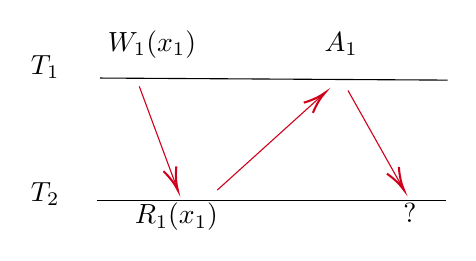
\begin{tikzpicture}[x=0.75pt,y=0.75pt,yscale=-1,xscale=1]
%uncomment if require: \path (0,300); %set diagram left start at 0, and has height of 300

%Straight Lines [id:da9500410641573396] 
\draw    (49.17,42) -- (216.56,43) ;
%Straight Lines [id:da7796185686481738] 
\draw    (47.56,101) -- (215.76,101) ;
%Straight Lines [id:da9563274467788809] 
\draw [color={rgb, 255:red, 208; green, 2; blue, 27 }  ,draw opacity=1 ]   (68,46) -- (85.86,94.13) ;
\draw [shift={(86.56,96)}, rotate = 249.64] [color={rgb, 255:red, 208; green, 2; blue, 27 }  ,draw opacity=1 ][line width=0.75]    (10.93,-3.29) .. controls (6.95,-1.4) and (3.31,-0.3) .. (0,0) .. controls (3.31,0.3) and (6.95,1.4) .. (10.93,3.29)   ;
%Straight Lines [id:da9159237520413861] 
\draw [color={rgb, 255:red, 208; green, 2; blue, 27 }  ,draw opacity=1 ]   (105.56,96) -- (156.08,50.34) ;
\draw [shift={(157.56,49)}, rotate = 137.89] [color={rgb, 255:red, 208; green, 2; blue, 27 }  ,draw opacity=1 ][line width=0.75]    (10.93,-3.29) .. controls (6.95,-1.4) and (3.31,-0.3) .. (0,0) .. controls (3.31,0.3) and (6.95,1.4) .. (10.93,3.29)   ;
%Straight Lines [id:da9009499956012581] 
\draw [color={rgb, 255:red, 208; green, 2; blue, 27 }  ,draw opacity=1 ]   (168.56,48) -- (194.58,94.26) ;
\draw [shift={(195.56,96)}, rotate = 240.64] [color={rgb, 255:red, 208; green, 2; blue, 27 }  ,draw opacity=1 ][line width=0.75]    (10.93,-3.29) .. controls (6.95,-1.4) and (3.31,-0.3) .. (0,0) .. controls (3.31,0.3) and (6.95,1.4) .. (10.93,3.29)   ;

% Text Node
\draw (14.5,30) node [anchor=north west][inner sep=0.75pt]   [align=left] {$T_1$};
% Text Node
\draw (51.56,18) node [anchor=north west][inner sep=0.75pt]   [align=left] {$W_1(x_1)$};
% Text Node
\draw (156,19) node [anchor=north west][inner sep=0.75pt]   [align=left] {$A_1$};


% Text Node
\draw (14.5,91) node [anchor=north west][inner sep=0.75pt]   [align=left] {$T_2$};
% Text Node
\draw (64.56,101) node [anchor=north west][inner sep=0.75pt]   [align=left] {$R_1(x_1)$};

% Text Node
\draw (194,101) node [anchor=north west][inner sep=0.75pt]   [align=left] {?};


\end{tikzpicture}
\vspace{2mm}
\begin{equation}
History\ H: [W_1(x_1),R_1(x_1),A_1,?]
\end{equation}
\vspace{2mm}
        \\

To prevent this: If a transaction has performed a read on an object modified by an aborted transaction, It itself has to abort.
\subsubsection{G1b: Intermediate Reads (Dirty Reads)}
    A history exhibits G1b if it contains a committed transaction containing a read of an intermediary modification by another transaction. i.e., a read of a non-final modification was performed and committed to the history. 
\tikzset{every picture/.style={line width=0.75pt}} %set default line width to 0.75pt        

\begin{tikzpicture}[x=0.75pt,y=0.75pt,yscale=-1,xscale=1]
%uncomment if require: \path (0,300); %set diagram left start at 0, and has height of 300

%Straight Lines [id:da9500410641573396] 
\draw    (62.09,31) -- (608.09,32) ;
%Straight Lines [id:da7796185686481738] 
\draw    (60.09,196) -- (606.09,197) ;
%Straight Lines [id:da424831019884359] 
\draw [color={rgb, 255:red, 198; green, 0; blue, 0 }  ,draw opacity=1 ]   (123.09,39) -- (175.41,185.12) ;
\draw [shift={(176.09,187)}, rotate = 250.3] [color={rgb, 255:red, 198; green, 0; blue, 0 }  ,draw opacity=1 ][line width=0.75]    (10.93,-3.29) .. controls (6.95,-1.4) and (3.31,-0.3) .. (0,0) .. controls (3.31,0.3) and (6.95,1.4) .. (10.93,3.29)   ;

% Text Node
\draw (13,10) node [anchor=north west][inner sep=0.75pt]   [align=left] {T\_490};
% Text Node
\draw (13,175) node [anchor=north west][inner sep=0.75pt]   [align=left] {T\_553};
% Text Node
\draw (85,9) node [anchor=north west][inner sep=0.75pt]   [align=left] {W(append 32 2)};
% Text Node
\draw (162,203) node [anchor=north west][inner sep=0.75pt]   [align=left] {R(32)};
% Text Node
\draw (298,203) node [anchor=north west][inner sep=0.75pt]   [align=left] {W(append 20 15)};
% Text Node
\draw (354,7) node [anchor=north west][inner sep=0.75pt]   [align=left] {Timeout on key 30};
% Text Node
\draw (531,203) node [anchor=north west][inner sep=0.75pt]   [align=left] {Commit};
% Text Node
\draw (122,133) node [anchor=north west][inner sep=0.75pt]   [align=left] {};
% Text Node
\draw (467,203) node [anchor=north west][inner sep=0.75pt]   [align=left] {R(30)};

\end{tikzpicture}


 \\
To prevent this, a: If a transaction has read an intermediate state of an object, it must be aborted, or an exclusive lock should be held to prevent other transactions from accessing an intermediate state.


\subsubsection{G1c: Circular Information Flow}
A history exhibits G1c if the DSG contains a directed cycle consisting entirely of dependency edges. There exist three possible combinations of such cycles: [ww,wr],[ww,ww],[wr,wr], below [wr,wr] is used for an example where T1 and T2 depend on eachothers writes.
\vspace{2mm}
\begin{figure}[h!]
\tikzset{every picture/.style={line width=0.75pt}} %set default line width to 0.75pt        

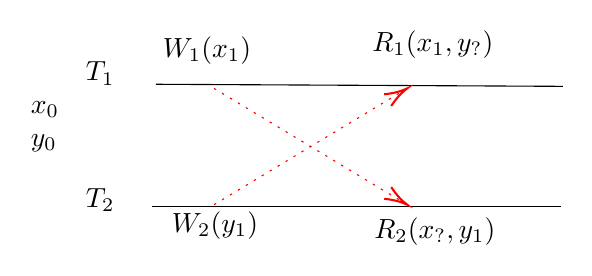
\begin{tikzpicture}[x=0.75pt,y=0.75pt,yscale=-1,xscale=1]
%uncomment if require: \path (0,300); %set diagram left start at 0, and has height of 300

%Straight Lines [id:da9500410641573396] 
\draw    (61.45,42) -- (257.56,43) ;
%Straight Lines [id:da7796185686481738] 
\draw    (59.56,101) -- (256.62,101) ;
%Straight Lines [id:da05192673528173475] 
\draw [color={rgb, 255:red, 255; green, 0; blue, 0 }  ,draw opacity=1 ] [dash pattern={on 0.84pt off 2.51pt}]  (89.56,100) -- (180.85,45.03) ;
\draw [shift={(182.56,44)}, rotate = 148.95] [color={rgb, 255:red, 255; green, 0; blue, 0 }  ,draw opacity=1 ][line width=0.75]    (10.93,-3.29) .. controls (6.95,-1.4) and (3.31,-0.3) .. (0,0) .. controls (3.31,0.3) and (6.95,1.4) .. (10.93,3.29)   ;
%Straight Lines [id:da10349511339666284] 
\draw [color={rgb, 255:red, 255; green, 0; blue, 0 }  ,draw opacity=1 ] [dash pattern={on 0.84pt off 2.51pt}]  (89.56,44) -- (180.85,98.97) ;
\draw [shift={(182.56,100)}, rotate = 211.05] [color={rgb, 255:red, 255; green, 0; blue, 0 }  ,draw opacity=1 ][line width=0.75]    (10.93,-3.29) .. controls (6.95,-1.4) and (3.31,-0.3) .. (0,0) .. controls (3.31,0.3) and (6.95,1.4) .. (10.93,3.29)   ;

% Text Node
\draw (26.5,30) node [anchor=north west][inner sep=0.75pt]   [align=left] {$T_1$};
% Text Node
\draw (26.5,91) node [anchor=north west][inner sep=0.75pt]   [align=left] {$T_2$};
% Text Node
\draw (165.56,105) node [anchor=north west][inner sep=0.75pt]   [align=left] {$R_2(x_?,y_1)$};
% Text Node
\draw (63.56,18) node [anchor=north west][inner sep=0.75pt]   [align=left] {$W_1(x_1)$};
% Text Node
\draw (68,102) node [anchor=north west][inner sep=0.75pt]   [align=left] {$W_2(y_1)$};
% Text Node
\draw (164.56,15) node [anchor=north west][inner sep=0.75pt]   [align=left] {$R_1(x_1,y_?)$};
% Text Node
\draw (0,49) node [anchor=north west][inner sep=0.75pt]   [align=left] {$x_0 $\\ $y_0$};
\end{tikzpicture}
\caption{G-1b cycle between $T_1$ and $T_2$, (wr, rw)}
\end{figure}
\vspace{2mm}
\begin{equation}
History\ H: [W_1(x_1),W_2(y_1),R_1(x_1),R_1(y_?),R_2(x_?),R_2(y_1),C_1, C_1]
\end{equation}
\vspace{2mm}

The above example has x and y in the initial state of 0, $T_1$ writes $x_1$ and $T_1$ writes $y_1$. They then read x,y. $T_1$ sees $x_1,y_0$ and $T_1$ sees $X_0,y_1$ while the actual state of the system is $x_1,y_1$


\subsection{G-Cursor: Lost Update}
A history exhibits G-cursor if the dsg contains a cycle with an anti-dependency (rw) edge and write-dependency (ww) edges using the same label.
\vspace{2mm}
\begin{figure}[h!]
\tikzset{every picture/.style={line width=0.75pt}} %set default line width to 0.75pt        

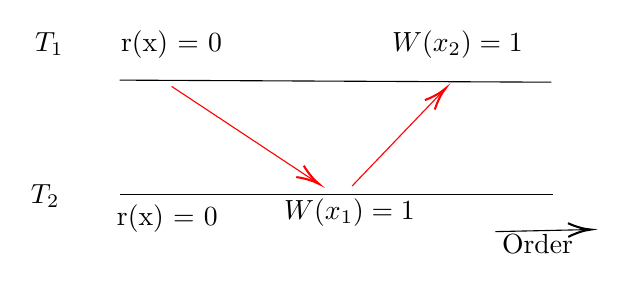
\begin{tikzpicture}[x=0.75pt,y=0.75pt,yscale=-1,xscale=1]
%uncomment if require: \path (0,300); %set diagram left start at 0, and has height of 300

%Straight Lines [id:da9500410641573396] 
\draw    (63.56,64) -- (271.56,65) ;
%Straight Lines [id:da7796185686481738] 
\draw    (63.56,119) -- (272.56,119) ;
%Straight Lines [id:da7329480179958066] 
\draw    (244.56,137) -- (288.56,136.04) ;
\draw [shift={(290.56,136)}, rotate = 178.75] [color={rgb, 255:red, 0; green, 0; blue, 0 }  ][line width=0.75]    (10.93,-3.29) .. controls (6.95,-1.4) and (3.31,-0.3) .. (0,0) .. controls (3.31,0.3) and (6.95,1.4) .. (10.93,3.29)   ;
%Straight Lines [id:da06917928011783969] 
\draw [color={rgb, 255:red, 255; green, 0; blue, 0 }  ,draw opacity=1 ]   (88.56,67) -- (157.89,112.9) ;
\draw [shift={(159.56,114)}, rotate = 213.5] [color={rgb, 255:red, 255; green, 0; blue, 0 }  ,draw opacity=1 ][line width=0.75]    (10.93,-3.29) .. controls (6.95,-1.4) and (3.31,-0.3) .. (0,0) .. controls (3.31,0.3) and (6.95,1.4) .. (10.93,3.29)   ;
%Straight Lines [id:da061796007668484476] 
\draw [color={rgb, 255:red, 255; green, 0; blue, 0 }  ,draw opacity=1 ]   (175.56,115) -- (219.18,69.44) ;
\draw [shift={(220.56,68)}, rotate = 133.75] [color={rgb, 255:red, 255; green, 0; blue, 0 }  ,draw opacity=1 ][line width=0.75]    (10.93,-3.29) .. controls (6.95,-1.4) and (3.31,-0.3) .. (0,0) .. controls (3.31,0.3) and (6.95,1.4) .. (10.93,3.29)   ;

% Text Node
\draw (21.5,40) node [anchor=north west][inner sep=0.75pt]   [align=left] {$T_1$};
% Text Node
\draw (19.5,113) node [anchor=north west][inner sep=0.75pt]   [align=left] {$T_2$};
% Text Node
\draw (141.56,120) node [anchor=north west][inner sep=0.75pt]   [align=left] {$W(x_1) = 1$};
% Text Node
\draw (63,39) node [anchor=north west][inner sep=0.75pt]   [align=left] {r(x) = 0};
% Text Node
\draw (246.56,137) node [anchor=north west][inner sep=0.75pt]   [align=left] {Order};
% Text Node
\draw (193.56,39) node [anchor=north west][inner sep=0.75pt]   [align=left] {$W(x_2)=1$};
% Text Node
\draw (61,123) node [anchor=north west][inner sep=0.75pt]   [align=left] {r(x) = 0};

\end{tikzpicture}
    \caption{G-Cursor cycle between $T_1$ and $T_2$, (wr, ww)}
\end{figure}
\vspace{2mm}
\begin{equation}
History\ H: [R_1(x_0),R_2(x_0),W_2(x=1),W_1(x=1)]
\end{equation}
\vspace{2mm}
\\
The above example has $T_1$ and $T_2$ performing a concurrent increment(x) call. $T_1$ and $T_2$ both read the initial state of $x=0$, $T_2$ then increments X via $W_2(x=1)$. $T_1$ then performs $W_1(x=1)$ overwriting the increment performed by $T_2$. The right outcome is $x = 2$

\subsection{G-Single: Read Skew}
A history exhibits G-single if the dsg contains a cycle consisting of an anti-dependency (rw) and dependency (ww, wr) edges.
\vspace{2mm}


\begin{figure}[h!]
\tikzset{every picture/.style={line width=0.75pt}} %set default line width to 0.75pt        

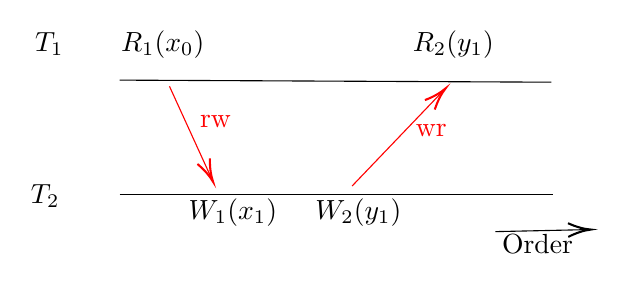
\begin{tikzpicture}[x=0.75pt,y=0.75pt,yscale=-1,xscale=1]
%uncomment if require: \path (0,300); %set diagram left start at 0, and has height of 300

%Straight Lines [id:da9500410641573396] 
\draw    (63.56,64) -- (271.56,65) ;
%Straight Lines [id:da7796185686481738] 
\draw    (63.56,119) -- (272.56,119) ;
%Straight Lines [id:da7329480179958066] 
\draw    (244.56,137) -- (288.56,136.04) ;
\draw [shift={(290.56,136)}, rotate = 178.75] [color={rgb, 255:red, 0; green, 0; blue, 0 }  ][line width=0.75]    (10.93,-3.29) .. controls (6.95,-1.4) and (3.31,-0.3) .. (0,0) .. controls (3.31,0.3) and (6.95,1.4) .. (10.93,3.29)   ;
%Straight Lines [id:da06917928011783969] 
\draw [color={rgb, 255:red, 255; green, 0; blue, 0 }  ,draw opacity=1 ]   (87.56,67) -- (107.73,111.18) ;
\draw [shift={(108.56,113)}, rotate = 245.46] [color={rgb, 255:red, 255; green, 0; blue, 0 }  ,draw opacity=1 ][line width=0.75]    (10.93,-3.29) .. controls (6.95,-1.4) and (3.31,-0.3) .. (0,0) .. controls (3.31,0.3) and (6.95,1.4) .. (10.93,3.29)   ;
%Straight Lines [id:da061796007668484476] 
\draw [color={rgb, 255:red, 255; green, 0; blue, 0 }  ,draw opacity=1 ]   (175.56,115) -- (219.18,69.44) ;
\draw [shift={(220.56,68)}, rotate = 133.75] [color={rgb, 255:red, 255; green, 0; blue, 0 }  ,draw opacity=1 ][line width=0.75]    (10.93,-3.29) .. controls (6.95,-1.4) and (3.31,-0.3) .. (0,0) .. controls (3.31,0.3) and (6.95,1.4) .. (10.93,3.29)   ;

% Text Node
\draw (21.5,40) node [anchor=north west][inner sep=0.75pt]   [align=left] {$T_1$};
% Text Node
\draw (19.5,113) node [anchor=north west][inner sep=0.75pt]   [align=left] {$T_2$};
% Text Node
\draw (156.56,120) node [anchor=north west][inner sep=0.75pt]   [align=left] {$W_2(y_1)$};
% Text Node
\draw (63,39) node [anchor=north west][inner sep=0.75pt]   [align=left] {$R_1(x_0)$};
% Text Node
\draw (246.56,137) node [anchor=north west][inner sep=0.75pt]   [align=left] {Order};
% Text Node
\draw (203.56,39) node [anchor=north west][inner sep=0.75pt]   [align=left] {$R_2(y_1)$};
% Text Node
\draw (95.56,120) node [anchor=north west][inner sep=0.75pt]   [align=left] {$W_1(x_1)$};
% Text Node
\draw (101,80) node [anchor=north west][inner sep=0.75pt]  [color={rgb, 255:red, 255; green, 0; blue, 0 }  ,opacity=1 ] [align=left] {rw};
% Text Node
\draw (205,84) node [anchor=north west][inner sep=0.75pt]  [color={rgb, 255:red, 255; green, 0; blue, 0 }  ,opacity=1 ] [align=left] {wr};


\end{tikzpicture}
    \caption{G-single cycle between $T_1$ and $T_2$, (rw, wr)}
\end{figure}
\vspace{2mm}
\begin{equation}
History\ H: [R_1(x_0),W_1(x_1),W_2(y_1),R_2(yx_1)]
\end{equation}
\vspace{2mm}
\\
In the above example $T_1$ observes $x_0$ and $y_1$ from various states of the system and therefor ended up reading an seeing inconsistent state. The two valid states in the above context is [$x_0$ , $y_0$] and [$x_1$ , $y_1$]

\todo[author=Mark]{Item Anti-dependency Cycles (write skew on disjoint read)}

\todo[author=Mark]{Add more DSG definitions if time permits.}
\newpage

\chapter{Consistency Model testing}

\section{Introduction}
Consistency model testing is the process of testing if a given system meets the requirement for a given consistency model. The way consistency models are defined is by which anomalies they prohibit. Therefore a straightforward method for testing whether a system meets the requirements for a model can be done by analyzing the transaction history for anomalies.\\
\vspace{5mm}
These tests are required to ensure that a system behaves expectedly and verify that they behave according to their creators' specifications. If a system does not behave as expected, situations can occur where information is lost, and harm can be done either bodily, financially, or materially. \\ \vspace{5mm}

In context, some transactional databases only allow for the execution of one transaction at a time where either the whole database or tables used are locked during transactions. In contrast, high-performance databases operate at a high concurrency level, allowing multiple transactions to operate on the same objects, thus allowing for higher performance and better scalability. However, these optimizations often have side effects due to poor implementation, understanding, or an intentional side effect to gain performance. These side effects might range from sometimes returning a stale value to the dirty reads and writes that allow for uncommitted data to persist. These side effects occur when allowing multiple processes to access or modify objects concurrently. Therefore, the system must ensure that the ordering of these operations does not violate the system's consistency model. For a system that does not operate concurrently, this is easily implemented. This same approach can be implemented via heavy locking for concurrent systems; however, this might lead to a high number of deadlocks and a consequent drop in performance, possibly lower than a nonconcurrent implementation. Instead, a scheduler is used to schedule and execute transactions concurrently. This scheduler is at fault for causing these violations, or rather optimizations of the scheduler. 
These circumstances arise when database creators attempt to improve the performance. During these optimizations, errors might inadvertently be introduced that allow for the execution of conflicting transactions. Therefore tests are required to check if a given optimization allows for conflicts.

\section{Historically}

Historically, testing was done using manually defined sets of transactions. They required careful consideration and were time-consuming to design, and often only able to check for simple patterns. These tests could check if a proven invariant held for a given consistency model or if an anomaly is present. They were also used to show if a system allowed long forks or snapshot isolation, and more importantly, at the time, if it supported them.

These tests are quite efficient but only check for specific patterns and therefore do not allow generalized checking if issues might be present. They were highly limited in what anomalies they could find and which consistency models they checked. Furthermore, due to the hard-coded and highly custom design, they are implemented on a system-to-system basis with no interchangeability.

This also means that the scope of these testing projects usually is enormous and defined case by case with predefined transactions that only test a limited scope. The test might have been done previously but was very limited in test coverage, and most anomalies were are never detected.

\section{State of the art}

Modern databases require automated testing suites to test if their behavior meets the requirements for their specification. During the investigating of what is available, three results were found, more possibly exist but not in the public space.
\begin{itemize}
\item Jepsen is an automized framework that allows for generalized consistency testing of nearly any type of system.
\item AGENDA\cite{AGENDA} is a partially-automatable tool that allows for ACID constraint testing. The only mention of this is in a paper from 2002 with minimal information available online. this is not fit for this use case as it does not allow for
\item HISTEX\cite{HISTEX} is a tool developed that allows for automated testing of a database but using hand-coded transactions and appears more in line with the historical way of performing consistency testing and can therefore not be used.
\end{itemize}

Of these three only Jepsen was suitable for use in this project.

\section{Jepsen}
Jepsen is a generalized consistency checker that works by performing black-box testing of a system via external observations of the transaction history. By its creator, Jepsen is presented as:
\begin{quote}
    "Jepsen is an effort to improve the safety of distributed databases, queues, consensus systems  (...) exploring particular systems' failure modes. In each analysis we explore whether the system lives up to its documentation's claims."\cite{jepsonio}
\end{quote}

\vspace{5mm}

Going from the above quote Jepsen is a way that allows us to check whether a given database system lives up to the requirements and premises that its creators give. Distributed systems are becoming common; this requires data storage to behave expectedly. The expected manner is used rather than the correct manner because we may allow certain faults to occur and allow for eventual consistency as this allows for higher throughput applications. There are cases where data may only be required locally to consider a transaction complete, even when some undesirable conditions occur. However, these are tolerated to a certain extent. \\

A scenario where real-time data distribution and correctness are of the utmost importance is within transactions in the finance industry, where we only want to consider a financial transaction committed once all shards of this data are replicated, and the 'old' balance is no longer available. Otherwise, we could reach a condition where worst case, a client can draw a negative balance on their account or where one of the transactions is not recorded as only one of the two transactions is recorded.\\

Oppositely a situation where eventual consistency is of no issues is for platforms like Facebook, YouTube, or Reddit. When a user comments on a post, this comment might not necessarily be available to users instantly, and it is of no concern if it takes a few seconds or minutes to be distributed to all nodes. Users generally do not notice these delays, and it allows for better scaling within these huge applications with mullions or billions of requests per second.\\

\vspace{5mm}

Jepsen, therefore, exists to test and check that systems behave expectantly. The way Jepsen performs these tests is to run clients externally of the target system. Hosts are connected via an IP network, and the clients are running on the same host in a single JVM instance, using the same driver to send requests to the system. The reason they are run in the same JVM is to ensure strict timekeeping of the requests. Clients then generate randomized operations and apply these over the network.

\vspace{2mm}
\begin{figure}[h!]
\tikzset{every picture/.style={line width=0.75pt}} %set default line width to 0.75pt        

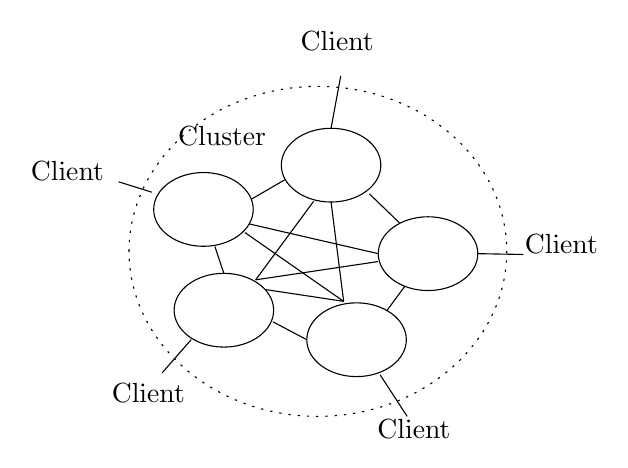
\begin{tikzpicture}[x=0.75pt,y=0.75pt,yscale=-1,xscale=1]
%uncomment if require: \path (0,724); %set diagram left start at 0, and has height of 724

%Shape: Ellipse [id:dp16650900496237675] 
\draw   (271.93,405.97) .. controls (271.93,396.15) and (282.66,388.2) .. (295.9,388.2) .. controls (309.14,388.2) and (319.88,396.15) .. (319.88,405.97) .. controls (319.88,415.78) and (309.14,423.73) .. (295.9,423.73) .. controls (282.66,423.73) and (271.93,415.78) .. (271.93,405.97) -- cycle ;
%Shape: Ellipse [id:dp685651119720939] 
\draw   (210.45,427.29) .. controls (210.45,417.48) and (221.19,409.52) .. (234.43,409.52) .. controls (247.67,409.52) and (258.4,417.48) .. (258.4,427.29) .. controls (258.4,437.1) and (247.67,445.06) .. (234.43,445.06) .. controls (221.19,445.06) and (210.45,437.1) .. (210.45,427.29) -- cycle ;
%Shape: Ellipse [id:dp7198461734461157] 
\draw   (318.65,448.61) .. controls (318.65,438.8) and (329.38,430.84) .. (342.62,430.84) .. controls (355.87,430.84) and (366.6,438.8) .. (366.6,448.61) .. controls (366.6,458.42) and (355.87,466.38) .. (342.62,466.38) .. controls (329.38,466.38) and (318.65,458.42) .. (318.65,448.61) -- cycle ;
%Shape: Ellipse [id:dp9105724275055453] 
\draw   (284.22,490.07) .. controls (284.22,480.26) and (294.96,472.3) .. (308.2,472.3) .. controls (321.44,472.3) and (332.17,480.26) .. (332.17,490.07) .. controls (332.17,499.88) and (321.44,507.84) .. (308.2,507.84) .. controls (294.96,507.84) and (284.22,499.88) .. (284.22,490.07) -- cycle ;
%Shape: Ellipse [id:dp08047780510308344] 
\draw   (220.29,475.85) .. controls (220.29,466.04) and (231.02,458.09) .. (244.26,458.09) .. controls (257.5,458.09) and (268.24,466.04) .. (268.24,475.85) .. controls (268.24,485.67) and (257.5,493.62) .. (244.26,493.62) .. controls (231.02,493.62) and (220.29,485.67) .. (220.29,475.85) -- cycle ;
%Straight Lines [id:da6784594846295133] 
\draw    (257.5,422.38) -- (273.53,413.06) ;
%Straight Lines [id:da07684116228139781] 
\draw    (314.38,419.79) -- (328.86,433.78) ;
%Straight Lines [id:da2065245145726602] 
\draw    (322.65,476.24) -- (331.44,464.33) ;
%Straight Lines [id:da6747154151499068] 
\draw    (267.84,481.42) -- (284.22,490.07) ;
%Straight Lines [id:da5547631888250106] 
\draw    (239.92,445.17) -- (244.26,458.09) ;
%Straight Lines [id:da7341618185433045] 
\draw    (287.49,423.42) -- (259.57,461.22) ;
%Straight Lines [id:da529005507481991] 
\draw    (318.65,448.61) -- (256.47,434.29) ;
%Straight Lines [id:da8601502324485646] 
\draw    (318.51,452.42) -- (259.57,461.22) ;
%Straight Lines [id:da1069842994819683] 
\draw    (295.9,423.73) -- (301.97,471.58) ;
%Straight Lines [id:da8033143862645027] 
\draw    (264.22,465.89) -- (301.97,471.58) ;
%Straight Lines [id:da38409352533043406] 
\draw    (254.4,438.44) -- (301.97,471.58) ;
%Shape: Ellipse [id:dp5026497859480832] 
\draw  [dash pattern={on 0.84pt off 2.51pt}] (198.56,447.5) .. controls (198.56,403.59) and (239.3,368) .. (289.56,368) .. controls (339.82,368) and (380.56,403.59) .. (380.56,447.5) .. controls (380.56,491.41) and (339.82,527) .. (289.56,527) .. controls (239.3,527) and (198.56,491.41) .. (198.56,447.5) -- cycle ;
%Straight Lines [id:da16909694919186213] 
\draw    (193.56,414) -- (209.56,419) ;
%Straight Lines [id:da7229592984672997] 
\draw    (214.56,506) -- (228.56,490) ;
%Straight Lines [id:da5812089250931924] 
\draw    (332.56,527) -- (319.56,507) ;
%Straight Lines [id:da14309192457407072] 
\draw    (388.56,449) -- (366.6,448.61) ;
%Straight Lines [id:da5613822733951459] 
\draw    (300.56,363) -- (295.9,388.2) ;

% Text Node
\draw (221,386) node [anchor=north west][inner sep=0.75pt]   [align=left] {Cluster};
% Text Node
\draw (150,403) node [anchor=north west][inner sep=0.75pt]   [align=left] {Client};
% Text Node
\draw (280,340) node [anchor=north west][inner sep=0.75pt]   [align=left] {Client};
% Text Node
\draw (388,438) node [anchor=north west][inner sep=0.75pt]   [align=left] {Client};
% Text Node
\draw (317,527) node [anchor=north west][inner sep=0.75pt]   [align=left] {Client};
% Text Node
\draw (189,510) node [anchor=north west][inner sep=0.75pt]   [align=left] {Client};


\end{tikzpicture}
\caption{Jepsen testing topology}
\end{figure}
\vspace{2mm}
\vspace{5mm}
The result from these operations can result in three outcome types. :ok, :fail and :info.
\begin{itemize}
\item :ok. The operation was executed as expected.
\item :fail. The operation failed and did not take place.
\item :info, an issue occurred in the system neither, this is cases of dropped connections, timeouts, or unknown exception. for these cases, it is assumed that the operation may or may not have happened or might occur later.
\end{itemize}
This history is used to reason about the state and order of the system and allows for checking for anomalies or other required properties. Linearizability can be checked by finding a path moving forward in time that touches every non-failed operation. If this path makes sense, i.e., we always read prior writes this history, this system is considered Linearizability. A dependency graph is built for serializable models, and violations are found by looking for cycles. \\

All of this functionality lies within the Jepsen client.

\subsection{Jepsen client}
The Jepsen client is built up in a modular fashion such that different modules perform specific tasks. This allows for delegation of responsibilities and allows modules to be reused. Different aspects of a test can be defined independently but may reuse a module instead and implementation overlapping functionality.

Generally, a Jepsen test suite consists of 5 modules. Database automation, client, generator, correctness checkers, and a fault introduction. On top of these modules, a test runner delegates tasks to each module.

\subsection{Runner}

The runner contains configurations for targets, rates, which faults should be introduced, and every other configurable aspect of the tests. This module also delegates tasks to other modules and which modules from the Jepsen libraries should be used. 

\subsection{Database Automation}
 The Database Automation or db module handles starting, stopping, and interaction with the database instance. Its main job is to spin up, prepare and configure the test target. This is not required for all tests, but it is best practice to do this as it allows for better repeatability of the tests. This module handles a vital feature of interacting with the instance once it runs, such as killing workers, causing crashes, removing the entire node from the cluster, or partitioning the network by manipulating the routing tables.

\subsection{Client}
The client executes a map of transactions via driver. It handles parsing, validation of return values, fault handling, and routing requests to the correct endpoint.

\subsection{Generator}
The generator's task is to generate the test map, which includes transactions and which and when to cause faults. It is also essential that the generator generates transactions that allow for the order of their execution to be deferred purely from external reads. Otherwise, correctness checking becomes much more difficult. 

\subsection{Correctness checker}
The checker module checks for anomalies in the resulting history; this can be a host of symptoms, out-of-order operations, violation of isolation, or corrupt data. 

\subsection{Fault inducer}
Nemesis is the module within Jepsen that generates faults; its task is to cause faults at random such as time skew, network partitions, crashes, increased package drop, or increased latency.


A scenario where real-time data distribution and correctness are of the utmost importance is within transactions in the finance industry, where we only want to consider a financial transaction committed once all shards of this data are replicated, and the 'old' balance is no longer available. Otherwise, we could reach a condition where worst case, a client can draw a negative balance on their account or where one of the transactions is not recorded as only one of the two transactions is recorded.\\

Oppositely a situation where eventual consistency is of no issues is for platforms like Facebook, YouTube, or Reddit. When a user comments on a post, this comment might not necessarily be available to users instantly, and it is of no concern if it takes a few seconds or minutes to be distributed to all nodes. Users generally do not notice these delays, and it allows for better scaling within these huge applications with mullions or billions of requests per second.



\subsection{Jensens internal modules.}
\subsubsection{Elle}
Elle,\cite{elle} inferring isolation anomalies from Experimental Observations. \\

Elle is a transactional consistency checker for black-box testing. It infers a dependency graph between client-side observations and the database version history. Checking is done via careful selection of database objects and operations such that database reads reveal information about the version history. Elle can therefore reveal anomalies and provide a concise explanation of why a fault occurred with information of what conditions were present during this fault. Using this information, we can state how a system behaves, what level of consistency, and which behavior we will see. This information can then compare the promises a system makes and how these promises are reflected in reality.\\
\vspace{5mm}


\section{Past Jepsen tests}
Jepsen.io contains publicly available test for 28 different systems. they nearly all contain issues or violation of the consistency model they are presented to meet. I will summarize the findings of a few prior tests below.
\subsection{Cassandra}
A test was done on Cassandra\cite{jepsencassandra} in 2013 that showed some interesting behavior; Doomstones, during conflicts, a lexicographically bigger value is winning. such that separate parts of separate transactions might persist in the database. .\\
\vspace{5mm}
Casandra itself is built on a hash ring via a distributed hash table like Service Fabric. Nevertheless, unlike most other databases, it uses timestamp-based last write wins. This allows for extremely high performance but also at the cost of being highly sensitive to clock skew.\\

In the test on Cassandra it was found that:
\begin{itemize}
    \item During a single key heavy write operation Losing 28\% of committed data and fails linearizable by any definition.
    \item During Write conflicts, roughly 1 in 200 rows end up being corrupt due to poor handling time where milliseconds are used with three zeros at the end instead of microseconds.
    \item \textit{No. Cassandra's lightweight transactions are not even close to correct. Depending on throughput, they may drop anywhere from 1-5\% of acknowledged writes–and this does not even require a network partition to demonstrate. It is just a broken implementation of Paxos. In addition to the deadlock bug, these Jepsen tests revealed \#6012 (Cassandra may accept multiple proposals for a single Paxos round) and \#6013, where an insert is rejected but committed. (unnecessarily high false-negative probabilities).}
\end{itemize}

\subsection{Postgres}
A Jepsen test\cite{jepsenpostgresql} was performed on PostgreSQL in 2020. During this test, several observations were made.
\begin{itemize}
    \item PostgreSQLs repeatable read behaves accordingly to snapshot isolation. G2-item violations occurred where write skew on disjoint read was observed ."
    \item PostgreSQLs serializability implementation contains the same issues, where concurrent update and insert transactions may exhibit G2-item.
\end{itemize}

\subsection{MonogoDB}

\begin{itemize}
\item In the first Jepsen test of MongoDB, 42% of writes were lost \cite{jepsenmongodb243}
\item In the second test of MongoDB, testing was done of its consistency model. It was found that MongoDB lies somewhere under Read Uncommitted\cite{jepsenmongodb267}
\item In the third test of MongoDB Lost updates, Dirty Reads, and Stale Reads was prevented with the v1 protocol. if the v0 protocol is used, these anomalies still occur.\cite{jepsenmongodb340}
\item The latest test of MongoDB tests claims about "full ACID transactions" where G-single (read skew), G1c (cyclic information flow), duplicated writes, and anomalies where a transaction could read its writes performed in the future. \cite{jepsenmongodb340}
\end{itemize}

\subsection{ElasticSearch}
In the jepsen test of ElasticSearch results showed that documents were lost due during a few scenarios.\cite{aphyrelasticsearch}
\begin{itemize}
    \item Intersecting partitions resulting in 2 primaries overwriting each other.
    \item Isolated primaries causing split-brain that is only recoverable by restart, however only one side of the clusters changes persisted.
    \item If the primary node pauses due to IO or garbage collection
\end{itemize}


\section{related work to Jepsen}

\todo[author=Mark]{ move these to BIB file and write this section}
% K. Kingsbury. Knossos.
% https://github.com/jepsen-io/knossos, 2013-2019.

% G. Lowe. Testing and Verifying Concurrent Objects.
% Concurrency and Computation: Practice and
% Experience, 29(4), 2017

% J. M. Wing and C. Gong. Testing and Verifying
% Concurrent Objects. Journal of Parallel and
% Distributed Computing, 17(1-2), 1993.

% P. B. Gibbons and E. Korach. Testing shared
% memories. SIAM Journal on Computing, 26(4), 1997

% S. Burckhardt, C. Dern, M. Musuvathi, and R. Tan.
% Line-up: A Complete and Automatic Linearizability
% Checker. PLDI '10, 2010.




    \newpage


    \chapter{Modern Datastores}

    The thesis will primacy focus on Service Fabrics. However, an investigation into other data stores is also done to allow comparisons and investigation into what different models affect the behavior of the database systems.


    \section{Service Fabric}

    \subsection{Introduction}

    Service Fabric (SF) is presented as a distributed systems platform akin to Kubernetes (K8S), where the user can build, deploy and scale microservices and containers. One of the key points presented by Microsoft on Azure Service Fabric is that developers are able to run stateful services. Microsoft presents it as the backbone of their core services and data stores.\\
    \vspace{5mm}

    \includegraphics[scale=0.5]{images/service-fabric-architecture.png}

    \subsection{System Architecture}

    The architecture behind Service Fabric is built via a layered approach; by Microsoft's words, this allows developers to write highly available applications, scalable, manageable, and testable. These layers are built on five Core and two supporting subsystems. Our main interest lies within the reliable collection, so we will only be investigating the layers and services that lay below this.\\
    \vspace{5mm}

    \subsubsection{Transport subsystem}
    \todo[author=Mark]{these might be serving the same purpose and the documentation might just be odd.}
    The lowest layer in the core stack provides secure communication within the cluster itself and between the cluster and clients. This functionality is provided via point-to-point communication channels that support one-way and request-reply patterns, in other terms UDP and TCP. This also provides the basis for broadcast and multicast within the cluster. Security is handled via either windows security or x509 certificates. \\
    \vspace{5mm}

    \subsubsection{Federation subsystem}

    The next subsystem in the stack is the Federation subsystem, which uses communication channels provided by the transport subsystem to gather the nodes into a unified service fabric cluster. It also provides system primitives that allow for Failure detection, leader Election and consistent routing within the cluster by upper layers in the system.\\
    \vspace{5mm}

    The core subsystem is built around an SF-ring developed internally at Microsoft in the early 2000s. Keys and nodes are mapped to points in the ring, with keys being owned by the node closest to it in the ring. Each node also uses this ring to keep track of its immediate successor and predecessor nodes in a Neighborhood set; the Federation layer then uses this set to run consistent membership and failure detection. Nodes also maintain long-distance routing partners that are used for consistent routing.\\
    \vspace{5mm}

    The membership and Failure detection are done using two key design principles.\\
    \vspace{5mm}

    Strongly Consistent membership and Decoupling Failure Detection from Failure Decision\\
    \vspace{5mm}

    \begin{itemize}
        \item \textbf{Strongly Consistent membership} All nodes monitoring the status of a given node must agree on whether the node is up or down. For use in the SF ring, this means that all nodes on the node's Neighborhood set must agree on its status.
        \item \textbf{Decoupling Failure Detection from Failure Decision}: Failure detection protocols can lead to conflicting states; therefore, the decision is decoupled from detection.
    \end{itemize}
    \vspace{5mm}

    To solve the issue of decoupling failure detection and decision-making on these failures. All decisions are distributed to a set of responsible nodes. This ensures that decisions are performed consistently and reliably. The detection of failures is performed via a distributed monitoring and leasing solution implemented in SF. This implementation solves this via Lease Renewal Request(LR) and LRack(Lease Renewal Acknowledgement). A node must maintain valid leases from all of its monitors, and these leases have to be renewed every lease period. This leasing period is calculated based on round trip times within the cluster. If a node fails to renew any of these leases, it considers removing itself from the set of nodes. If a monitor misses a lease request to a node, the node turn considers marking the monitor as failed. Both of these decisions need to be approved by an Arbitrator group. If a node fails to receive an LRack within a timeout based on round trip time, it repeats the LR until it receives an LRack. Due to the nature of the SF-ring, these monitor relations are symmetrical, but this Lease protocol is still run independently. There are other cases; if a node fails the renewal process, it stops renewing leases to any other nodes, or if a node detects another node as having failed, it stops sending renewal requests to it. These 2 cases can cause inconsistencies if they were operating alone; however, deciding if a node is down or up is up to the Arbitrator group, which maintains consistent memberships. \\
    \vspace{5mm}

    The Arbitrator group performs the decision to determine failures. This is separate from the neighborhood set. They operate independently, and it has two ways of deciding if a given node has failed. The way that the groups stay consistent when members join or leave the group is that when an Arbitrator joins the set, it initially rejects all requests in the first T seconds. This is done to prevent new Arbitrators from making conflicting decisions with the excising nodes and prevent failed nodes from existing in the distributed membership protocol. This ensures that detected nodes leave before being forgotten.\\
    \vspace{5mm}

    \begin{enumerate}
        \item X detects Y as failed and sends fail(Y) to the arbitrator
        \item The arbitrator adds Y to a recently failed list and sends ack(fail(y)) containing a timeout for Y to X. If The arbitrator already marked X as having failed and ignores the request,
        \item If X receives this request, it waits for the timeout to claim Y's ring area. Moreover, if it receives no response within the timeout, it leaves itself.
    \end{enumerate}

    If a node is already in the recently failed list, it returns the same response as the first reporter, except it calculates the time since the first detection, so the neighbors claim the portion of the ring it owns at the same time. This also means that the routing can continue after time out with a laxity added. All routing requests for a node are added to a queue if a node is marked as failed. The queue is then released after Timeout+laxity that allows all neighboring nodes to claim that part of the ring and allows these routing requests to be performed by its successors.\\
    \vspace{5mm}

    If the case of two nodes reporting each other failed, the conflict is resolved either by a majority; the node that was reported first to the most Arbitrators leaves the ring. A second option is to heal the membership if both nodes are healthy and can therefore stay. \\   \vspace{5mm}
    
    The implementation in SF is presented as failure tolerant towards cascade failures as the decision is not made by the detectors themselves but by arbitrators.
    This can be in cases of network congestion or -partitions that result in multiple nodes detecting each other as failed. For traditional distributed hash-tables, this can result in membership list or ring inconsistencies.\\ 
    \vspace{5mm}

    \includegraphics[scale=0.3]{images/servicefabric-fig-ring-topology.jpeg}

    \paragraph{SF-Ring and consistent routing}

    The Distributed Hash table used for Service Fabric routing is an evolution of SF-ring developed within Microsoft in the 2000s. The routing used offers symmetry, and due to this, it allows bidirectional routing that allows for lookup and routing via binary search. This allows SF to quickly route messages around the ring, with multiple routing options. There are always two routing partners on either side of the destination that help distribute the load and route, even with stale routing tables. Initially, all packages were routed using this method; this has changed over the years. Today the hash table is used to build a routing table and maintain it when a new node is added to the cluster. After discovery, a direct route is used via the destination IP address. \\
    \vspace{5mm}

    Routing tables work differently depending on the size of the cluster. However, it can route in two ways. If the size of the routing table is smaller than the number of nodes a direct route is used, if there exist more nodes in the cluster than the routing tables, it switches to routing via routing tables to reduce memory consummation but causing an increase in time complexity to O(log(n)) from O(1)\\
    \vspace{5mm}
    \paragraph{Routing Tokens}
    
    Each node owns a token that includes a portion of the routing token it is responsible for. The SF-ring protocol ensures two properties:
    \begin{itemize}
        \item Each token is only owned by one node at any given time;
        \item Eventually, every token is owned by one node.
    \end{itemize}
    This ensures SF handles nodes joining and leaving the ring. Initially, a bootstrap node owns the entire ring. After the initial bootstrap node, any joining node will split the ring segment between them. Routing tokens are also used for leader election, simply the owner of a given key is the owner. This same process ensures that no keys are abandoned.

    \subsubsection{Reliability subsystem}
    The reliability subsystem is in charge of load balancing, replication, and availability. These three aspects are provided via three services: a Failover Manage, a Naming and Resolution, and a Placement, and lastly, a Load Balancer service.\\
    \vspace{5mm}

    The Failover Manager runs as a stateful service with an instance running on each node in the cluster that provides three actions: start a replica, move a replica, and reconfigure a replica.\\
    \vspace{5mm}

    \begin{itemize}
        \item \textbf{Create a replica} Create a new replica when instructed by the PLB
        \item \textbf{Move a replica} migrate a replica when instructed by the PLB to a different node.
        \item \textbf{Reconfiguration} If a primary replica becomes unavailable, promote a secondary as the new primary. If the old primary comes back only, it is demoted to secondary.
    \end{itemize}

    A service called Failover Master Manager is also running that can restart the failure manager via a cached state in case it fails. If the master fails, it can rebuild its state via the SF-ring. The Master Failover manager is running on the node whose token range contains ID0.\\
    \vspace{5mm}

    The naming and resolution service map instance names to endpoints that services are listening on. This allows for consistent routing from outside the cluster via URI that does not change over their lifetimes.\\
    \vspace{5mm}

    The Placement and Load Balancer(PLB) service is stateful and is in charge of placing replicas and instances of services on nodes and ensures an even load throughout the cluster. They claim that, unlike other solutions where services are hashed onto the ring in SF, the PLB explicitly assigns each service replica Primary and Secondary nodes in the ring. It continually monitors the cluster for available resources. This allows for assignment and migration of services to underutilized nodes; more importantly, it ensures services are migrated away from a node that is about to enter a service window or in cases of over-utilization that could lead to service degradation\\
    \vspace{5mm}

    The technique used for selecting the placement of nodes is done via Simulated Annealing, as it is presented to provide a near-optimal solution as to where services can be placed. The way the system is modeled is via resource use in the system where an even load is desired, but some constraints need to be met, such as fault tolerance, avoiding replica co-location, and some services might have a strict set of nodes to run on. \\
    \vspace{5mm}

    \subsubsection{Reliable Collections}

    Reliable collections provide stateful services in Service Fabric via Reliable Directories and Reliable Queues that are available for C\# and Java programming and are promised to be:
    \begin{itemize}
        \item Available and Fault-tolerant via replication,
        \item Persistent via disk
        \item Efficient via asynchronous via a nonblocking API.
        \item Transnational via APIs with ACID semantics.
    \end{itemize}

    One of the key differences between storage systems built on SF and other highly-available systems is that states are kept locally in the replica while also being made highly available. This causes most reads to be local.\\
    \vspace{5mm}

    Writes are relayed from the primary replica to secondary replicas via passive replication. A write is considered complete when the majority of secondaries acknowledge it. The relaxations allow an application to achieve weaker consistency by relaxing where a read can go, e.g., always write to primary and read from secondary. \\
    \vspace{5mm}

    SF is presented as the only "self-sufficient microservice system that can be used to build a transactional consistent database which is reliable, available, self-*, and upgradeable because the lower layers assure consistency"\cite{SFpaper} \\
    \vspace{5mm}

    \paragraph{Consistency models/isolation levels}
    SF reliable collections promise two Select-able consistency models that the user can pick. Repeatable Read and Snapshot Isolation. \todo[author=Mark]{maybe delete this last line.}eg, there is no promise about Serializability of the transactions.\\
    \vspace{5mm}

    \begin{table}[h]
        \centering
        \begin{tabular}{l|l|l}
            & \multicolumn{2}{c@{}}{\text{Role}} \\
            \text{Operation}   & Primary         & Secondary \\
            Single Entity Read & Repeatable Read & Snapshot  \\
            Enumeration, Count & Snapshot        & Snapshot
        \end{tabular}
        \caption{Isolation level defaults for Reliable Dictionary and Queue operations.}
        \cite{SF_RC_Transactions}
    \end{table}


    \section{Programming for Service Fabric}
    
    Development for the Service Fabric Framework closely resembles the development flow for Dotnet Web applications and Kubernetes service development. There are however, tighter constraints where the application is only executable in azure as no local development environment exists for Linux. \\
    
    Writing the code itself is possible via either Java or C\#. Documentation only really exists for C\#. However, this documentation also seems outdated and lacks quite a bit of information. Generally, an MVC application is the best choice for the architecture of the service itself, where stateless or stateful variants are available.\\
    
    Debugging and testing code on the Linux implementation is highly lacking, with no debug tooling available such as remote executing with a debugger or support for dump files to analyze crashes and issues within the application. This caused development to be slow-paced, trail\&error and draining. I would recommend creating a working application before integrating the Service Fabric functionality. On top of this, using heavy logging from the application to an external store allows for insight.
   \\
   A careful note here should also be taken as there is no features parity between platforms which causes core functionality to be unavailable on Linux.



\section{Comparison}
In many of the papers published by Microsoft, many comparisons are made to Cassandra, Redis, and Dynamo. Therefore, an introduction will be made to two of these as they are comparable in many aspects. The investigation will not be as deep as with SF, but consistency and failure modes will be investigated.

    
    
\subsection{Cassandra}

One of the systems that Microsoft draws comparisons to is Casandra. Casandra was initially made by Facebook and later made open-source via the Apache Software Foundation. It uses the same underlying distributed hashtable to form a Ring; however, unlike Service Fabric, Casandra is leaderless to allow for greater scalability and is purely a database. it handles transactions and operations in a Last Write Wins consistency model. This implementation makes it sensitive to time desync and Clock skew where the wrong value might persist. Its use cases are mainly within instant messaging, where values are written and rarely modified but must be distributed quickly. 

Failure detection is done via a gossiping channel and a sliding value. The way failures are handled is that nodes avoid querying a failed node's value to reach the threshold; this threshold is dynamically adjusted based on network and load conditions. Memberships of a cluster are explicitly initiated by an administrator who manually performs the addition and removal of nodes from a Cassandra instance.\cite{Cassandra}
    
    

    \subsection{Redis}
\todo[author=Mark]{write section on Redis}



    \section{Comparison}
\todo[author=Mark]{write Comparison between the 3 datastores}
    In many of the papers published by Microsoft a lot of comparisons are made to Cassadra, Redis and Redis. Therefore, comparisons will be made to these as they are comparable in a lot of aspects. The investigation won't be as deep as with SF but investigation of consistency and failure modes will be be done.


    \chapter{Jepsen Test on Service Fabric Reliable collections}

    One of the goals of the thesis was to attempt to perform a Jepsen test on Service Fabric Reliable Collections subsystem. Reliable Collections powers services in Azure and is the target of this endeavor. 
    This chapter will present the design, implementation, and revisions of the testing suite. \\
    \vspace{5mm}
    To perform such a test, we need to build up both a testing suite, APIs, and libraries to connect the Jepsen service and the Service Fabric core components. Therefore, a few different applications and services need to be learned, understood, designed, implemented, tested, executed, and finally, the data generated can be analyzed.
    

    \section{Design \& implementation}
    The Design of the services required for preforming the Jepsen test were revised multiple times following a a learn by during methodology as I did have no prior experience with Service Fabric, Jepsen, C\# or Clojure. 

    \subsection{Initial Design}

    The initial design of the testing suite contained two applications. The first one is a Service Fabric application containing a stateful and a stateless Service. The second application is a Clojure application running the Jepsen testing suite.

    \subsubsection{Service Fabric Services}

    The Service Fabric stateless service contains endpoints our Jepsen test can interact with. These should then be routed to the correct stateful service partition. The initial design contained endpoints for insert, Add, Update, Check\&set, delete, and Delete All, which operated on a reliable directory datatype. The service is implemented using C\# as the lack of documentation for Service Fabric for Java made this seem like the better choice (as of writing, nearly all this documentation is for the C\# language). Both services will expose these endpoints via the Kestrel web server. This was made as it is the native implementation already integrated into SF, had the most documentation, and was therefore deemed the safest choice to proceed with.\\
    \vspace{5mm}
    A flow diagram for the design of the stateful service contains the following functionality. The Stateless service works as a forwarding service as it is simply a 1:1 mapping with partition calculations for use in the routing of the request. \\
    \vspace{5mm}
    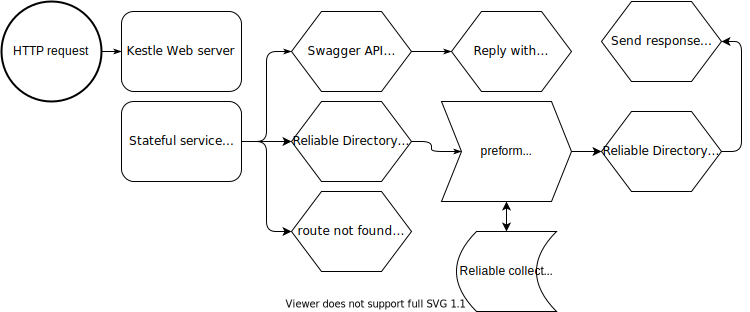
\includegraphics[scale=0.5]{images/Design_Stateful_service_1.0.drawio.png}
    \todo[author=Jacopo]{missing description of this figure. What are these components? Time allowing provide some text explaining what this figure is supposed to say}

    This implementation contains two primary codebases. The C\# dotnet web services act as an API to the reliable collections using three controllers for the three default data structures implemented in the framework and a Clojure codebase containing the Jepsen test and a driver for connecting to the Service fabric services.

    \subsection{Infrastructure}
    The infrastructure is centered around Azure, using an isolated v-net containing six virtual machines running Linux. Ubuntu was chosen because it is a known distribution that we are familiar with. one of the six nodes runs the Jepsen application, while the five remaining notes run the Service Fabric Cluster.
    The 5 Service Fabric nodes are managed by Service fabric, and the configuration is deployed to them via Azure. There are cases where manual intervention is required due to the cluster becoming unhealthy and is unable to heal. in these cases, a full reimage of the cluster is performed. ,  Applications can be deployed via either the Azure Service Fabric CLI \cite{servicefabriccli} or via Visual Studio \cite{servicefabricguide}. The latter was the process used during the development stages of the project.

    The Jepsen host is manged and accessed via ssh. A deployment pipeline was considered but was decided against due to development overhead. A solution using SCP was chosen instead due to the quicker development cycles and that only a single machine required access to the deployment. 
    

    The network's topology is arranged such that the six nodes are located in the same VLAN to keep connections local and prevent outside connections from causing issues with the test.\\
    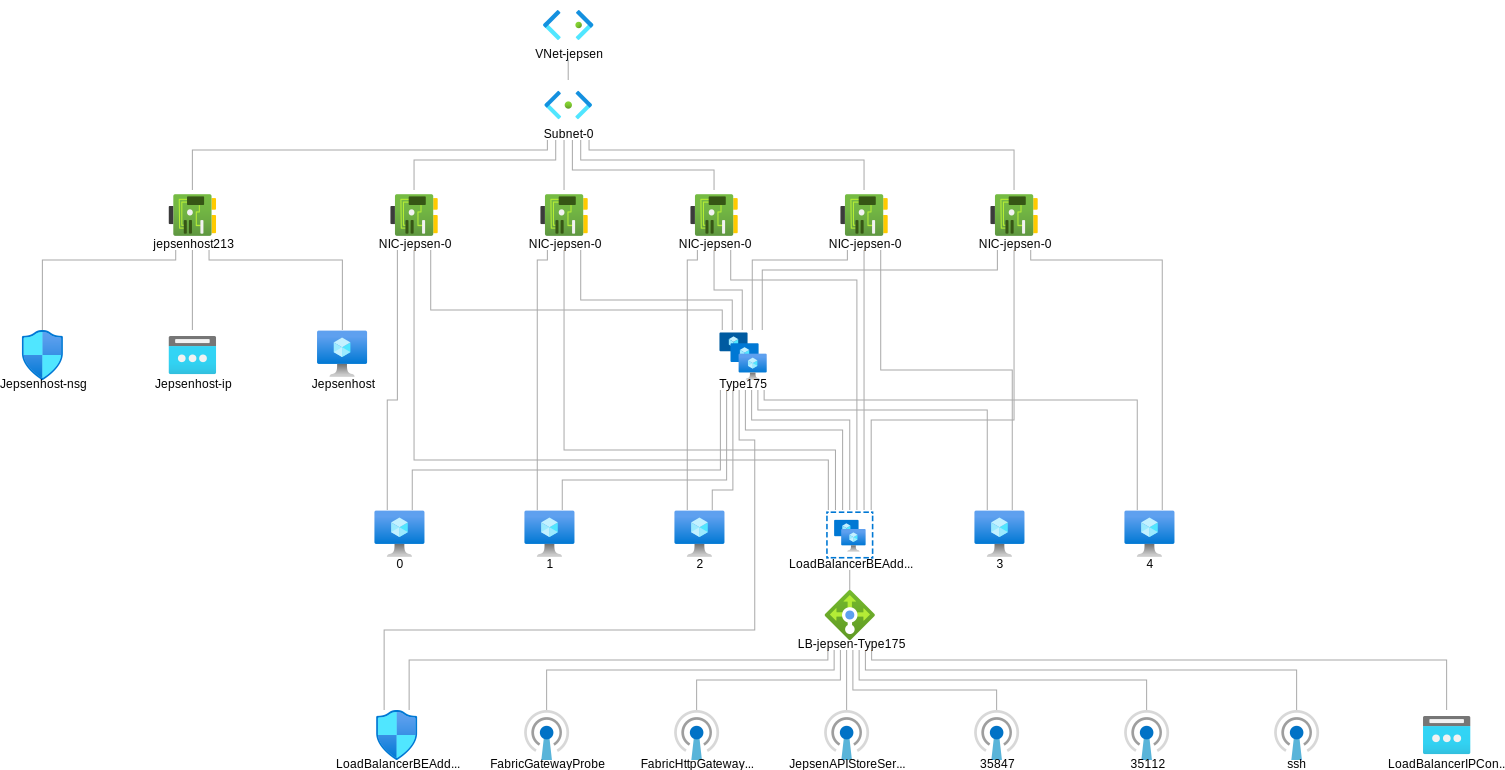
\includegraphics[scale=0.3]{images/topology.png}
    \\
    \todo[author=Jacopo]{missing description of this figure. What are these components? Time allowing provide some text explaining what this figure is supposed to say}

    All traffic resides within the cluster. The load balancer is part of the standard service fabric deployment and allows for connection to the management interface, deployments, and access to the underlying hosts. These endpoints were protected by firewall rules that only allowed connections from approved sources to avoid external influence on the results.

    \subsubsection*{Node Sizes}

    The initial node size contained 2vcpu, 8 GBs of ram, and 20 GB of local storage, as this was thought to be enough to handle the workload of the test. This was later revised as the nodes had issues with disk space and often took a long time to set up and get ready for any given deployment. This problem was resolved by upgrading the size of the nodes to 4vcpu, 16GB Ram, and 80GB local storage per node. This configuration resulted in a more well-behaved cluster. This node size was kept for the remainder of the project. However, the Jepsenhost is slightly under-dimensioned compared to its handling when analyzing the test result. This is primarily due to out-of-memory errors that could be solved by lowering the test's search space or increasing the node's memory.


    \subsection{Services}
    As mentioned earlier, running these tests required multiple components. The stateful service that hosts the reliable collections from SF Reliability subsystem, a stateless front-end that provides this data to clients via an API, a driver that handles the connection to this API, and finally the Jepsen test suite itself consisting of workloads, generator, checker and Nemesis module.

    \subsubsection{SF services}
    Microsoft recommends using two services, such that a Stateful service is never directly exposed to the internet but where a stateless service acts as a proxy. This provides multiple benefits but also a few negatives. The prime benefit is abstracting from the back-end and adding a layer of validation, routing, and protection of the back-end service. Time connections are held open should also be reduced to due round trips times being lower, which should allow for higher throughput.

    \paragraph*{Stateful Reliable collection service}

    The stateful services provide three separate controllers that expose one of the built-in reliable collection data types, These three being: Reliable Dictionary, Reliable Queue, and Reliable Concurrent Queue. Faults are also handled at this stage where faults caused by transactional issues are returned to the client via HTTP status codes\cite{wikihttpstatuscodes}: node not primary, accepted, result not found, and internal server error. This should allow for more straightforward diagnoses and handling of faults when parsed by the Clojure application.

    The fronted stateless service provides these same APIs but with wrappers and routing in a portioned design. This layer could also be used to build additional features, but this was not the case as only the bare transactions supported by the reliable collections layer were needed.

    \paragraph*{Jepsen test suite}
    
    The design of the Jepsen test suite aims to use skeleton code from a past Jepsen test to start the project as it gives a template of what functionality should be implemented. These implementations are still custom, but it gives a pointer to the bare minimum of a functioning application.
    \\
    The first module is a Driver that allows our test to connect to our stateless API. Options here are to either write it in Java or Clojure. An attempt will be made to implement this in Java, but Clojure might be the choice depending on implementation issues or compatibility issues. This module should handle connections, exceptions and parse values in both directions.\todo[author=Jacopo]{did you use Java or Clojure. Here write the final result, not speculation.}
    \\
    The Jepsen suite should use a modular setup that allows interoperability between multiple workloads, a runner that allows for test tuning, db that deploys, configures, and operates on the running datastore; a client runs the transactions via the driver, a nemesis that induces faults in the cluster and three workloads, queue, concurrent queue, and dictionary. One workload for each of the transactional data types exposed by Service Fabric.
    \begin{itemize}
        \item The runner module is the main class. It handles defaults, CLI input, and workload selection along with the configuration of common behavior shared between workloads, nemesis, db, and other mutual features for all workloads.
        \item   The db module should handle spinning up and tearing down the services along with functions for stating, stopping, and killing services and workers in the cluster.

  \item  The nemesis modules should contain the functions that kill, partition, or in other ways introduce failures in the cluster.

  \item 3 workloads act on different data types, each requiring a separate generator, checker, and client.
    \end{itemize}
    
    Only one should be used for the final testing of the three workloads designed. They should all exhibit the same symptoms if issues exist, but all three are initially implemented to decide which type should be focused on.
    

  
\subsubsection{Implementation of the initial design}

The initial design targeted the reliable collection dictionary datatype. It presented a few issues with the design and implementational details that were not considered. The biggest obstacle when developing for Service Fabric is the non-feature parity between Linux and the Windows implementation; this is caused by two parallel implementations where some core functionality is not yet available in the Linux implementation. This resulted in unfavorable conditions with no debugging support, dump files that were not readable, lack of documentation, and black box behavior as local code execution was impossible. \\ \vspace{5mm}
A large amount of time was spent debugging, changing configuration files, stripping any unneeded libraries, and rolling back to older versions of frameworks used. It should be noted that the Service Fabric framework was kept at the same release while .NET and similar aspects were rolled back to older releases.

However, all of these attempts were frugal, after two months deleting all code and restarting from scratch using a different approach. An attempt was made via an implementation via Java, which was also unsuccessful, and finally went back to C\#. After getting a working solution for the project on a Service Fabric Cluster running on a Windows host, I reached out to Mikkel Hegnhøj from Microsoft for assistance.

The issue turned out to be twofold.
\begin{itemize}
    \item .NET needing to be rolled back to 3.5
    \item The entry point has to be defined via .NET and the name of the DLL file. As documented in the official doc, I attempted something like this by using an entry point via a bash script. 
\end{itemize}

Finally, I had a working version on Linux, or rather, I had a way to run the application on Linux as the issues did not stop here. The Feature parity was still there. The DNS routing service is missing from the Linux implementation; this required endpoints to be hardcoded, where each service was bound to a given port. This introduced a limit of 1 replica of a given service per node. This dramatically reduces horizontal scaling as we need an extra node per partition. Running larger partitions on each node is also an option. However, from a performance, availability, and reliability perspective, having lots of smaller partitions is much more effective than one large database instance that introduces higher risks of deadlocking and other issues.


\paragraph*{Implementation details SF}

The design uses a stateless service that processes the incoming request and routes it to a back-end service. The get key endpoint will be used to outline the design. All the stateless endpoints closely resemble each other; therefore, only this will be included here.\\
        
\paragraph*{Stateless Service}
The Stateless service is implemented via Model View Controllers (MVC) that expose the website via a kestrel web server. Each endpoint route is defined via flags which define protocol and request type followed by paths and an endpoint name. A HTTP get request using a path variable as a parameter, The \textbf{"[HttpGet("{key}")]"} flag is used. This is then followed by a function that allows the MVC design pattern, but this function is an Async function that takes the key as a variable and returns a \textbf{"Task<IActionResult>"}. The used return type allows for the return value to be either JSON or predefined methods to return bad requests, No Content, or other HTTP response codes without requiring explicit handling.
\begin{lstlisting}[language=csh]
public async Task<IActionResult> Get(string key)
\end{lstlisting}   

The underlying Service Fabric framework exposes an endpoint used to retrieve all partitions of a given stateful service. This is coupled with the internal routing in the transport subsystem, such that any service in the cluster can easily and securely be found and reached. 
\begin{lstlisting}[language=csh]
    ServicePartitionList partitions = await this.fabricClient.QueryManager.GetPartitionListAsync(serviceName);
\end{lstlisting}   
This allows us to query the individual partitions, where any aggregate operations are handled in the stateless service.
\begin{lstlisting}[language=csh]
    foreach (Partition partition in partitions)    {  .. Do something ..  }
    return result;
\end{lstlisting}  
\paragraph*{Stateful Service}

The stateful service was implemented via the MVC patterns and followed a design that kept simplicity in mind where each endpoint exposed and performed one operation and committed this change to the datastore. This allowed for querying the database quickly and consistently, even if data split among partitions.
\begin{lstlisting}[language=csh]
        [HttpGet("{key}")]
        public async Task<IActionResult> Get(string key){
        ...
         while (await enumerator.MoveNextAsync(ct)){
                  if (enumerator.Current.Key == key)
                  { return this.Json(;(enumerator.Current);
    }}}
\end{lstlisting}   

\paragraph*{Implementation details Clojure}
During the initial implementation of the Jepsen test, quite a few aspects were somewhat chaotic. Programming practices do not carry over from object-oriented programming into dynamic and functional programming. The Clojure programming language was treated as a learn by doing. This resulted in the first implementation of the application functioning, but not without issues. Most of these were a cause of not fully understanding the language used and how the information flowed within it. This caused issues with HTTP requests being mishandled and responses not being parsed correctly into the history such that transactions with a status of failed were considered valid in the history used to check the consistency of the model.
 
This caused the whole application to exhibit a broad range of unintended and weird behavior, resulting from asynchronous distributed systems being complex and concurrent applications handling 100s or 1000s of threads requiring careful planning and considerations.
       
       
The Clojure application itself is split into different modules that expose classes. the core modules required to make up a Jepsen test suite require a runner, generator, Nemesis (a type of Chaos monkey)\cite{Choasmonkey}, db, client, connector/driver, and workloads.
\begin{itemize}
   \item The \textbf{Runner} contains the majority of the configurations and a CLI interface that exposes options and settings where generalized values for the tests are specified. This is also where a select Workload is chosen for running the test. Three different workloads were implemented that each required a generator, checker, client, and Nemesis.
       
  \item  The \textbf{Generator} class generates a list of transactions to execute, which can later be used to check the transaction history for any anomalies. This is closely linked with the checker.
       
  \item  The \textbf{checker} checks for anomalies in the transaction history, This could be by either checking if all committed values exist in the data store after the test, if there are transactional violations in the data store, if odd behavior like the case of Casandra where multiples objects are merged due to conflicts that might lead to an unintended outcome. 
       
 \item  the \textbf{client} interface maps the generated list of transactions to the driver calls for a given data store. This module processes the map generated by our generator into transactions, parses the transaction into a format the driver understands and back into a format Jepsen understands as well as handling any errors, exception as well as basic check if the operation failed and succeeded and logs this to the internal transaction history handled by Jepsen.
\end{itemize}
       
The Jepsen application required a driver to be written for Clojure to interact with the API exposed by the stateless service; This could have been written in either Java or Clojure. An attempt was made to implement this in Java with some success but was scrapped, and implementation was done in Clojure instead. The driver performs HTTP/HTTPS calls to the service fabric cluster and handles input validation, connection management, fault handling of connection, and parsing any faults and results returned by the service into a format compatible with Clojure.
       

\subsubsection{Resolving issues with the design.}
   

The initial version of the service fabric has some issues with the stateless service. Due to a high number of connections from the Jepsen host, the connection buffer overflow caused issues for connections between the stateless service and the underlying state-full services that provided the data.

A few considerations on how this issue could be resolved were considered, lowering the latency between nodes in the cluster, removing the stateless layer, and connecting directly to the stateful service. A choice here was made to scrap the initial implementation for Service Fabric and redesign it only to require a stateful service. The transactions would behave the same in a  single partition compared to a cluster with 500 partitions, as each "primary" node will behave the same, either way with the implementation that service fabric exposes. The service should therefore have a primary node as well as a few active replicas that allow for checking of replication status if this should be required down the line. This resolves and simplifies two things. Routing to the separate partitions is no longer an issue as the stateless "proxy" node is removed, we no longer need to consider routing data to the correct node from our Clojure connector, where it is possible to route all traffic to the primary or only route writes to the primary while distributing the reads to check for replication issues. This allows for testing of the replication engine in the future.

\subsubsection{implementation of the revised design}

The implementation of this \todo[author=Jacopo]{I lost it. what is this revised design? The structure of this chapter is not clear. You jump talking about designs. You should clarify that you are talking about the initial design early and then move to the final design. Now is very confusing.} revised design was supposed to be fairly straightforward. However, the lack of feature parity started causing issues. These started showing up after an update to a new version of Service Fabric, a change to the behavior of warning to instead throw errors. This exposed the inexperience working with the .Net framework and the service fabric framework. These issues were eventually ironed out, but a significant amount of time was again lost due to the lack of debugging support either from a local cluster or diagnostic output from the cluster running in azure. This turned the development cycle upside down as there is no way to execute the code without a Service Fabric cluster.
\\ \vspace{5mm}
Nevertheless, the code would not run on the Service Fabric cluster due to an error code that lacked definition or documentation. The issue here was related to changes in allowed port ranges that were not allowed to be used by services, port 80 and port 443. The applications were therefore killed. These warnings were not displayed correctly in the Linux distribution so\todo[author=Jacopo]{so?} tweaking code and settings while scouring the internet was the only apparent solution for these issues.

\paragraph*{Implementation changes for the SF Application}
The second iteration of the Service Fabric application removes the stateless layer of the application. These changes aimed to increase the throughput by removing a layer of network traffic and routing. This required moving the request handling, parsing, and verification to the stateful service.   \\

The changes required here were not overly complex and only required merging the code and ensuring that only valid data was used in transactions. 
\\

\paragraph*{Implementation changes for the Clojure Application}
This design iteration did not require any significant changes to the Clojure application. The changes were only on the routing side of Service Fabric. This did require minor changes to the connector such that the headers of the requests such that\todo[author=Jacopo]{such that (and as always dots not followed by capital letter} they were valid as internal service fabric requests. Otherwise, the connections from the Clojure application were rejected by the stateful application. Routing is defined such that the primary node is connected to by default. This should probably have been implemented as a command-line configuration, but the immediate solution was chosen as that endpoint would have to be defined either way. 


\subsubsection{Final iteration of the design.}
At this point in the process, a significant flaw was realized and required significant changes to how transactions were handled. In other words, the generator, checker, driver, and client had to be rewritten on the Clojure side, and most of the code on the Service Fabric side required the same treatment. 
\\
The prior Designs treated the system as a BASE data store. We performed single operation transactions, where multi-operation transactions to test the transactional data store, where a transaction can contain an arbitrary long ordered list of operations to execute. 
\\
A change was made to the network topology. All nodes were added to a proximity group that should reduce any latency or keep it to a minimum and ensures that outside forces such as bottlenecked routing or switching gear do not affect the test results.  \\


\paragraph*{Stateless service}

The changes required for the Service fabric cluster required changing how transactions were passed to the service before URI path variables were used. For transactions requiring multiple operations, this is not viable. The API was changed to accepting a transaction stored in JSON via URI parameters. This allows for greater flexibility and a standardized way to pass information and configuration between the two services if needed. 

This should be implemented by parsing the incoming transaction JSON into an iterable format and iterating over it, performing the required sub-operations of a given transaction, and committing afterward.

\paragraph*{Clojure application}

The Jepsen application requires significant redesign. Centered around the generation of transactions instead of sub-operations, Starting with the driver where the choice is to add a new interface that requires new code that handles transactions instead of sub-operations, On top of the Driver layer, the Client module sits, for this, a change in design is required that handles the new data type, complexity added by it. It should parse the incoming transactions pass this on to the driver, where verification and fault handling should occur when a result or exception is returned. The generator should generate transactions containing a list of operations. Here, the Jepsen Elle module provides functionality that eases the generator's implementation and the checking for the generated ordering.

\subsubsection{Implementation of the final design}

\paragraph*{Stateless service}

The changes to the stateless services required designing a new API endpoint that collected all functionality of the existing endpoints. For the implementation use of tools such as Postman, dotnetfiddle, and curiousconcept JSON tool was used. This allowed testing concepts and code ideas before implementing them for the Service Fabric cluster. The implementation was still time-consuming due to the lack of debugging tools and generally black-box behavior of Service Fabric. Stemming from the inability to run the application locally, the cluster returned internal server codes that were not usable for debugging the solution. The issue here turned out to be wrong documentation, which ended up requiring a few days of investigation prior to solving the issue. It also summarizes the entire development process so far.\\ \todo[author=Jacopo]{ be aware that this can also be read as "I can not read the documentation good enough. Note that often the failures are hidden in the final work. Here you chose to describe the failures in every step, but this can also give the image to the external reviewer of someone that can not do the job properly"}

Solutions such as implementing application logging or application performance monitoring could have given insight into why the application did not behave as expected. Looking at many things in hindsight, plenty of poor decisions were made that would be changed, and the whole design mythology of the project might be done differently.\todo[author=Jacopo]{this are consideration better to do in the conclusion}

\vspace{5mm}

The JSON data passed to the Jepsen service is of the following format, It's simply parsable into native JSON were any desired operation can be preformed on it. There were some issues with formatting where Service Fabric crashed due to non handled characters in the payload, or occasions where some text values where denoted correctly leading to crashes. \\
\begin{lstlisting}[language=json]
{  "transaction":[
{      "operation":"Enqueue",
 "key":"Key123",
 "value":456456    },
{      "operation":"Dequeue",
 "key":"Key123"    },
{      "operation":"abort"      }  ]}
\end{lstlisting}  

The revised stateless service uses the transaction JSON by parsing it into a native JSON object in .Net and loops over it and checks for operation types, simply executes them according to the type, and ads the result of the operation to a result list.
\begin{lstlisting}[language=csh]
[HttpPut]
public async Task<IActionResult> Put(){
    ....
       foreach (var item in transaction.operations)
            {if (item.operation.type == "read")
                {conditionalValue = await reliableDictionary.TryGetValueAsync(tx, item.key.Value);
                        result.Add(new KeyValuePair<string, string>(item.key.Value, value.ToString()));}
            ....
     await tx.CommitAsync();
     return this.Json(result);}
\end{lstlisting}  

In the case of exceptions, the cases are handled by a try-catch that returns the state of the transaction as aborted along with why a given transaction was aborted to allow for later analysis.

\paragraph*{Implementation changes to the Jepsen Clojure application.}


The changes to the Jepsen application required starting anew of many of the modules. In places where this was viable, these changes were implemented as a parallel execution path in case the older code might be relevant; in other cases, the older code was discarded in favor of the new implementation.
\\
\vspace{5mm}
An entirely new implementation of the driver was required. The modules receive a Clojure Map that is parsed into JSON verifying the transaction's validity; This payload is then packed into a get request where relevant metadata is added. A check is first performed on the returned payload to handle any exceptions or errors. Secondly, a check is performed to check the transactions commit status. If it is aborted or ended in a different failure, and lastly, if the return status is good, the return values are parsed and returned to our Client module.
\\
\vspace{5mm}
The Client Module was restarted to handle multi-operation transactions. Here the module's requirement was the implementation of code to handle preparing the map and checking and verifying the values returned from the driver. The payload is prepared by parsing the Clojure map into a JSON-compatible format. When retrieving the data, it should verify the values, check the status of the returned value, and store the returned values in our history for later analysis.
\\
\vspace{5mm}
    
The changes for the Generator and checker shifted a lot of the heavy lifting from custom generators and Checkers into using Elle, where the generated transactions are unique to ensure traceability. The checker then uses these unique values to check for phenomena via directed serialization graphs rules.
\\
\vspace{5mm}

\subsubsection{Running the test}

The testing suite is run in Azure using six nodes. Five for service fabric and 1 for the Jepsen host. Service Fabric is in charge of the cluster for Orchestration. Deployment of the applications to the cluster is pretty trivial and can be done either via Visual studio or a PowerShell script; The Jepsen test code is deployed to the Jepsen node test node. The Jepsen node can connect to the 5 Service Fabric nodes via SSH to induce crashes, time skew, and other failures and issues. During the test, the systems take care of themselves. Depending on the length of the test, the tester can either remain connected during the test and follow the tail of the output or reconnect later to retrieve the results. The test outputs Client-side transaction logs containing all issues and results from the test enriched with issues found by the checker. This means the test data can be analyzed with different tools or manually checked for issues not covered by automatic testing.

\todo[author=Jacopo]{how long do they run, how many times have you repeated them. If someone has to reproduce what you did, he or she will have a hard time understanding what to do with such a scarce description}


\subsubsection{Issues during the Design and implementation stages.}

Service Fabric Linux and Windows versions of the framework are far from interchangeable,\todo[author=Jacopo]{english!} This results in applications and services that function on one version failing on the other. This especially presented issues as the local development environment provided by Microsoft might write an application, but the same application would fail to run or crash on the cluster. This issue was further concatenated by Visual Studio being unable to load dump files that would allow a debugger to trace why the applications from the cluster were not functioning as intended. Other debugging options, such as the remote debugger feature, were not compatible with the Linux cluster, which meant we were often flying blind during the development. There were also some minor issues with the cluster becoming unhealthy/corrupt and nodes not being configured correctly after a re-image that required an entirely new deployment of the cluster and any data that might have been in the cluster to be lost. This was not an issue for this experiment but could have been significant issues in a production scenario with data not redundantly stored on a different data store.

\newpage
\section{Results}

\subsection{Introduction}

The results from the experiment using Jepsen to check whether Service Fabric Living up to the promises presented by Microsoft the below findings were made. 
\begin{itemize}
    \item The consistency provided by Service fabric does not live up to the isolation guaranteed provided by Repeatable read as promised by Microsoft. Service Fabric does also not make use of the relaxations permitted by this consistency model, In the sense that it handles locking poorly, resulting in deadlocks and timeouts.
    \item Contains :G1a, :G1b, :G0 violation most ACID Consistency models.
\end{itemize}



\subsection{Consistency model results.}
The Consistency model results show that Service Fabric does not live up to the requirements for read-atomic and read-committed. From this, it can be deduced that any stricter consistency models are also not met. Due to this, this is part of the disheartening results from the Jepsen test. 
\begin{lstlisting}
:not #{:read-atomic :read-committed},
:also-not #{
:ROLA,:causal-cerone,:consistent-view,:cursor-stability,:forward-consistent-view
:monotonic-atomic-view,:monotonic-snapshot-read,:monotonic-view
:parallel-snapshot-isolation,:prefix, :repeatable-read, :serializable
:snapshot-isolation,:strict-serializable,:strong-session-serializable
:strong-session-snapshot-isolation,:strong-snapshot-isolation,:update-serializable
}
\end{lstlisting}

\newpage
\subsection{Violation of the Consistency models}
\subsubsection{G0: Dirty Write}

Dirty Writes are pretty common as soon as conflicts occur within Service Fabric. In the included example, transaction 21005 has been aborted after performing a write to key 249 while waiting for a shared lock for key 251. during this process 100 starts transaction 21019 by writing to key 249 followed by a read to this same key. The Violation is that the write from transaction 21005 should not be readable prior to being committed. However during transaction 21019, this key is read and updated with the dirty changes from 21005 and the new value from 21019. key 249 is then read containing both the values 15 and 27.

    
\vspace{2mm}
\tikzset{every picture/.style={line width=0.75pt}} %set default line width to 0.75pt        

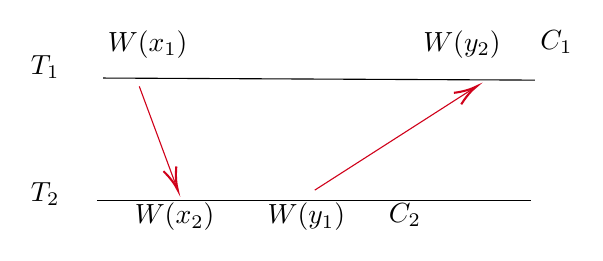
\begin{tikzpicture}[x=0.75pt,y=0.75pt,yscale=-1,xscale=1]
%uncomment if require: \path (0,300); %set diagram left start at 0, and has height of 300

%Straight Lines [id:da9500410641573396] 
\draw    (50.56,42) -- (258.56,43) ;
%Straight Lines [id:da7796185686481738] 
\draw    (47.56,101) -- (256.56,101) ;
%Straight Lines [id:da9563274467788809] 
\draw [color={rgb, 255:red, 208; green, 2; blue, 27 }  ,draw opacity=1 ]   (68,46) -- (85.86,94.13) ;
\draw [shift={(86.56,96)}, rotate = 249.64] [color={rgb, 255:red, 208; green, 2; blue, 27 }  ,draw opacity=1 ][line width=0.75]    (10.93,-3.29) .. controls (6.95,-1.4) and (3.31,-0.3) .. (0,0) .. controls (3.31,0.3) and (6.95,1.4) .. (10.93,3.29)   ;
%Straight Lines [id:da9159237520413861] 
\draw [color={rgb, 255:red, 208; green, 2; blue, 27 }  ,draw opacity=1 ]   (152.56,96) -- (228.88,47.08) ;
\draw [shift={(230.56,46)}, rotate = 147.34] [color={rgb, 255:red, 208; green, 2; blue, 27 }  ,draw opacity=1 ][line width=0.75]    (10.93,-3.29) .. controls (6.95,-1.4) and (3.31,-0.3) .. (0,0) .. controls (3.31,0.3) and (6.95,1.4) .. (10.93,3.29)   ;

% Text Node
\draw (14.5,30) node [anchor=north west][inner sep=0.75pt]   [align=left] {$T_1$};
% Text Node
\draw (51.56,18) node [anchor=north west][inner sep=0.75pt]   [align=left] {$W(x_1)$};
% Text Node
\draw (203.56,18) node [anchor=north west][inner sep=0.75pt]   [align=left] {$W(y_2)$};
% Text Node
\draw (260,18) node [anchor=north west][inner sep=0.75pt]   [align=left] {$C_1$};


% Text Node
\draw (14.5,91) node [anchor=north west][inner sep=0.75pt]   [align=left] {$T_2$};
% Text Node
\draw (64.56,101) node [anchor=north west][inner sep=0.75pt]   [align=left] {$W(x_2)$};
% Text Node
\draw (128.56,101) node [anchor=north west][inner sep=0.75pt]   [align=left] {$W(y_1)$};
% Text Node
\draw (187,101) node [anchor=north west][inner sep=0.75pt]   [align=left] {$C_2$};
\end{tikzpicture}
\vspace{2mm}

\begin{lstlisting}
{:key 249,
:values [15 27],
:txns [{:type :fail,
        :f :txn,
        :value [[:append 249 15] [:r 251 nil]],
        :time 204766434560,
        :process 18,
        :error Timed out waiting for Shared lock on key;",
        :index 21005}
       ...
       {:type :ok,
        :f :txn,
        :value [[:append 249 27]
                [:r 249 [1 2 3 7 8 11 15 27]]],
        :time 204800363164,
        :process 100,
        :index 21019}]}
\end{lstlisting}

\newpage
\subsubsection{G1a: Aborted Reads (cascaded aborts)}
Aborted reads are common as they share the same underlying issues as Dirty Update. These occur when a transaction commits that it has read the updates of an aborted transaction.\\

The below example. Transaction 336 wrote to key two and afterward aborted due to being unable to retrieve a lock on key 24. this write was read in Transaction 754, which should not have been possible.

\begin{figure}[h!]
\tikzset{every picture/.style={line width=0.75pt}} %set default line width to 0.75pt        

\begin{tikzpicture}[x=0.75pt,y=0.75pt,yscale=-1,xscale=1]
%uncomment if require: \path (0,300); %set diagram left start at 0, and has height of 300

%Straight Lines [id:da9500410641573396] 
\draw    (62.09,31) -- (608.09,32) ;
%Straight Lines [id:da7796185686481738] 
\draw    (60.09,196) -- (606.09,197) ;
%Straight Lines [id:da424831019884359] 
\draw [color={rgb, 255:red, 198; green, 0; blue, 0 }  ,draw opacity=1 ]   (123.09,40) -- (396.34,191.03) ;
\draw [shift={(398.09,192)}, rotate = 208.93] [color={rgb, 255:red, 198; green, 0; blue, 0 }  ,draw opacity=1 ][line width=0.75]    (10.93,-3.29) .. controls (6.95,-1.4) and (3.31,-0.3) .. (0,0) .. controls (3.31,0.3) and (6.95,1.4) .. (10.93,3.29)   ;

% Text Node
\draw (14,10) node [anchor=north west][inner sep=0.75pt]   [align=left] {T\_336};
% Text Node
\draw (13,175) node [anchor=north west][inner sep=0.75pt]   [align=left] {T\_754};
% Text Node
\draw (85,9) node [anchor=north west][inner sep=0.75pt]   [align=left] {W(append 22 3)};
% Text Node
\draw (216,204) node [anchor=north west][inner sep=0.75pt]   [align=left] {R(23)};
% Text Node
\draw (399,205) node [anchor=north west][inner sep=0.75pt]   [align=left] {R(22)};
% Text Node
\draw (403,10) node [anchor=north west][inner sep=0.75pt]   [align=left] {Abort due to timeout};
% Text Node
\draw (531,173) node [anchor=north west][inner sep=0.75pt]   [align=left] {Commit};
% Text Node
\draw (122,133) node [anchor=north west][inner sep=0.75pt]   [align=left] {};


\end{tikzpicture}

\caption{G1a: Aborted Reads violation that occurred during one of the runs.}
\end{figure}

\begin{lstlisting}
    {:op {:type :ok,
        :f :txn,
        :value [[:r 23 [4 5]]
                [:r 22 [1 2 4 3 5 30 32]]],
        :time 10926481665,
        :process 180,
        :index 754},
   :mop [:r 22 [1 2 4 3 5 30 32]],
   :writer {:type :fail,
            :f :txn,
            :value [[:append 22 3]
                    [:append 24 7]],
            :time 6857604069,
            :process 8,
            :error "Timed out waiting for Exclusive lock on key",
            :index 336},
   :element 3}
\end{lstlisting}



\newpage
\subsubsection{G1b: Intermediate Reads (dirty reads)}
Dirty reads occur when a process reads a change prior to this change being committed. 

In the below example.
Transaction 490 writes a change to key 32. this change is then read, which is committed prior to 490 committing/aborting.


\tikzset{every picture/.style={line width=0.75pt}} %set default line width to 0.75pt        

\begin{tikzpicture}[x=0.75pt,y=0.75pt,yscale=-1,xscale=1]
%uncomment if require: \path (0,300); %set diagram left start at 0, and has height of 300

%Straight Lines [id:da9500410641573396] 
\draw    (62.09,31) -- (608.09,32) ;
%Straight Lines [id:da7796185686481738] 
\draw    (60.09,196) -- (606.09,197) ;
%Straight Lines [id:da424831019884359] 
\draw [color={rgb, 255:red, 198; green, 0; blue, 0 }  ,draw opacity=1 ]   (123.09,39) -- (175.41,185.12) ;
\draw [shift={(176.09,187)}, rotate = 250.3] [color={rgb, 255:red, 198; green, 0; blue, 0 }  ,draw opacity=1 ][line width=0.75]    (10.93,-3.29) .. controls (6.95,-1.4) and (3.31,-0.3) .. (0,0) .. controls (3.31,0.3) and (6.95,1.4) .. (10.93,3.29)   ;

% Text Node
\draw (13,10) node [anchor=north west][inner sep=0.75pt]   [align=left] {T\_490};
% Text Node
\draw (13,175) node [anchor=north west][inner sep=0.75pt]   [align=left] {T\_553};
% Text Node
\draw (85,9) node [anchor=north west][inner sep=0.75pt]   [align=left] {W(append 32 2)};
% Text Node
\draw (162,203) node [anchor=north west][inner sep=0.75pt]   [align=left] {R(32)};
% Text Node
\draw (298,203) node [anchor=north west][inner sep=0.75pt]   [align=left] {W(append 20 15)};
% Text Node
\draw (354,7) node [anchor=north west][inner sep=0.75pt]   [align=left] {Timeout on key 30};
% Text Node
\draw (531,203) node [anchor=north west][inner sep=0.75pt]   [align=left] {Commit};
% Text Node
\draw (122,133) node [anchor=north west][inner sep=0.75pt]   [align=left] {};
% Text Node
\draw (467,203) node [anchor=north west][inner sep=0.75pt]   [align=left] {R(30)};

\end{tikzpicture}


\begin{lstlisting}
  :G1b ({:op {:type :ok,
        :f :txn,
        :value [[:r 32 [1 2]] 
                [:append 20 15] 
                [:r 30 [5]]],
        :time 18957901065,
        :process 71,
        :index 553},
   :mop [:r 32 [1 2]],
   :writer {:type :fail,
            :f :txn,
            :value [[:append 32 2] 
                    [:append 30 9] 
                    [:r 16 nil] 
                    [:append 30 10] 
                    [:append 32 3]],
            :time 14930759485,
            :process 84,
            :error "System.TimeoutException: Timed out waiting for Exclusive lock on key",
            :index 490},
   :element 2})},
\end{lstlisting}


\newpage
\subsection{Rejected transactions}

One of the symptoms that the reliable collections showed was ever-increasing abort rates for transactions containing more than one operation. These aborts were caused by heavy deadlocking and timeouts, bringing the entire system to a slowdown with test parameters of 200 concurrent clients and randomly distributed transactions with 1-10 sub-operations aborting 89.5 \% of the time, meaning only 10.5 \% of the transaction got committed. The reason for these aborts resolves around how the API to service fabric is designed, which causes it to be blocking. The reliable collection does not perform any query optimizations or checks prior to acquiring a lock or attempting to acquire them. 

With 100 concurrent connections, the following abort rates were found. 

\begin{figure}[h!]
\begin{tikzpicture}
\begin{axis}
[
    xlabel={Transaction length}, 
    ylabel={Abort rate in \%}, 
    grid, 
    xmin=0, 
    xmax=11, 
    ymin=0, 
    ymax=100
]
\addplot[red, mark=x, smooth] table[col sep=comma]{results/dataresult.csv};

\end{axis}
\end{tikzpicture}
\caption{Abort rates during 10 test with concurrency 100 with "max txn length" ranging from 1 to 10}
\end{figure}

\chapter{Discussion}

During this thesis, a surprising amount of information was found in existing papers, both concerning databases in general. The lack of precise and unambiguous definitions surrounding them, coupled with the number of database systems that violate the consistency models they are presented to follow. This point also applies to service fabric where violations occur with aborted transactions persisting, and deadlocks cause a high number of aborts due to the lack of query optimizations within Service Fabric.\\ \vspace{5mm}

    \begin{itemize}
        \item Learning the required tools to implement the services and applications in the first place. C\#, Clojure, and Service Fabric itself and reliable collections and lastly Jepsen itself.
        \item Understanding the problem, requirement, topology, architectures, and how we want to test these things.
        \item Designing the Services, Libraries, APIs, testing suite, the infrastructure and networking of the cluster and azure.
        \item Implement the Services, Libraries, APIs, and testing suite required for things to talk to each other.
        \item Test all the code and configurations and ensure things work as intended.
        \item Execute the test itself.
        \item Analyse the data from the test.
    \end{itemize}
    

\section{Consistency model Standards or the lack thereof}

Before this thesis, databases were always presented as fairly strict, adhering to strict behavior with predictable results. This turned out to lack a few asterisks where the definitions for databases behavior are ambiguous. Many databases often fail these requirements when they are put under some workloads. Some of the more worrying findings are how often Nosql databases lose data and how often SQL databases violate their set consistency model. This is also not a discovery either. Looking at papers over the past ten years, it is a topic that is being investigated more and more. It also appears that changes are first being made when a third party in the open-source community brings these issues to light. The paper from Haixiang et al. \cite{li2021coo} is one of the more recent papers that summarize existing literature on the topic. Coo, like many papers prior to the definition of Consistency models, not in terms of things they prohibit but in unambiguous mathematical notation that cleanly defines what can and cannot be expected.\\
\vspace{5mm}
This unambiguous definition would prevent the current situation where databases are presented differently compared to how they behave in reality. Currently, mislabeling and misclassification of databases are the norm. This issue will persist with no standardized way to classify or test them, like aborted reads in Service Fabric or the other issues discovered while working on the thesis. \\\vspace{5mm}
\begin{itemize}
    \item Postgres concerning its implementation of repeatable read or its replication functionality.
    \item MongoDB dropping data and violating consistency models.
    \item Casandra last-write wins issues
    \item Elastic search losing data.
\end{itemize}

These issues can have huge implications in the real world. Often this behavior is not well understood by the users of the systems. Just here in Odense, MongoDB is used by the city to gather data from intersections, water usage, water height levels, temperatures, pollution, and many other metrics and data points around the city. In this use case, these issues might only annoy a few city planners and other city officials. Situations might occur where these systems are used in a critical application. i.e., in Healthcare, where no data loss is acceptable, medical journals with data critical to human life could be lost due to the information. This case could be due to the system not behaving as expectedly or system designers choosing a system without understanding its behavior.

\section{How can this be improved going forward}

There is no single way to resolve all of the issues surrounding the definitions of consistency models. These issues stem from the ANSI\cite{ansisql1999} standard where due to poor official definitions, either other definitions are used, or these definitions are used that allow for the flaws within them. Information should be available to ensure that developers to ensure that they understand the tradeoffs of a given systems consistency model. System implements should also use automated testing to ensure expected behavior. Such that any issues are found before being shipped and deployed. \\
\vspace{5mm}
Students should be taught about transaction models and use cases during introductory database courses where behavior is explained to prevent misuse of consistency models where they do not belong. This should not be in-depth, but Read Uncommitted or last-write-wins databases are fine for logging. However, they should be avoided for certain use cases due to their behavior.\\
\vspace{5mm}
Industries should define a standard for testing and checking database systems towards a consistency model. Such a standard would allow the industry to homogenize the labeling, allowing users and developers to choose the current system for their use case and avoid the headaches of anomalous behavior.

\section{Results from Service Fabric}

The results from the experiment show the violation of the consistency models presented by Microsoft. In the results, 3 Types of violations were found; Dirty Write, Dirty Read, and Intermediate Read. Furthermore, no use of the consistency models relaxations. Service Fabric instead uses a strict locking approach; a large number of deadlocks occur, resulting in timeouts and what was supposed to have aborted transactions. It appears that when an exception is thrown, it should be strictly handled; otherwise, the keys are unlocked, and other transactions can access the dirty values. According to the documentation, such events are handled by the system aborting, and users should restart the transaction\cite{servicefabricguidelines}
However, it appears that this is not the case. a modified implementation of the Service Fabric Stateful service was implemented that manually handled the case of lock timeout seems to resolve the serializable issues in Service Fabric.\\
\vspace{5mm}
The poor use of allowed optimizations is harder to solve. Service fabric does not run a scheduler to optimize the ordering of operations; instead, these are run in the order executed by a given process. The only way to allow for these optimizations would be to handle the execution transactions at a lower level, Either via a new module or interfaces that allow for serialization of all concurrent transactions.

\chapter{Conclusion and Outlook}
\section*{Conclusion}

In this thesis, we presented some of the currently used consistency models. How they are defined, what is wrong with the current definitions, and how the scientific community and industries have tried to address these shortcomings. No standard body has yet rectified the flawed definitions used in standards such as Ansi\cite{ansi}. 
Following this initial study, Jepsen was presented. Independent parties from the open-source community created Jepsen. Jepsen was developed due to the mislabeling of current systems. It allows for testing whether a given system meets the requirement for behavior prevented by its creators or what flaws a system exhibits in general. 
Following the presentation, a Jepsen Service Fabric was presented. Service Fabric is a  distributed systems platform designed by Microsoft. It contains a system for providing distributed transactional data types. 
Using the knowledge gained from the above sections, Jepsen was used for conducting a test on Service Fabric. The results of this test were that Service Fabric violates the Repeatable read consistency model by allowing uncommitted transactions to persist when exceptions interrupt their execution. 
Lastly, a discussion on the current state of consistency models, definitions, or the lack thereof, what implications this has, and what can be improved things going forward. Here the finders are the new industry standards required that rectify ambiguous definitions and a system for testing systems towards this standard.



\section{Future Work}

Future work could include implementing a deeper testing suite that checks for more types of invariant and issues that might occur in the system.


\newpage
\chapter{Appendix}

\pagestyle{empty}
\printbibliography


\section{Proposal}
\input{Proposal}

\section{Revised Proposal}
\section{'Jepsen methods usage for consistency compliance testing in Hyperscale Cloud Frameworks (Updated due to 3 month extension)'}

\section{Introduction}
The goal of this project is to assess how Jepsen\footnote[1]{https://aphyr.com/tags/jepsen } tests allow us to verify the properties of ACID\footnote[2]{Database Management Systems by Raghu Ramakrishnan \& Johannes Gehrke  ISBN13 9780071231510} in a cloud system.
The Jepsen test is a method used to evaluate the compliance of a system in relation to the ACID properties. This is done is by analysing the system via Blackbox\footnote[3]{https://youtu.be/tRc0O9VgzB0?t=293} tests , in the sense that the internals of the system work are not relevant. We look at the service from a client-side and not any underlying structures or frameworks.
The ACID\footnote[2]{Database Management Systems by Raghu Ramakrishnan \& Johannes Gehrke  ISBN13 9780071231510} properties are 
\begin{itemize}
\item	Atomicity \\
Guarantees that each transaction is treated as a single "unit", which either succeeds completely or fails completely 
\item	Consistency \\
Ensures that a transaction can only bring the database from one valid state to another
\item	Isolation \\
Ensures that concurrent execution of transactions leaves the database in the same state that would have been obtained if the transactions were executed sequentially 
\item	Durability \\
Guarantees that once a transaction has been committed, it will remain committed even in the case of a system failure 
\end{itemize}
 \\
We plan to apply these methods on Service Fabric\footnote[4]{https://docs.microsoft.com/en-us/azure/service-fabric/service-fabric-overview  } , to verify if this system is compliant with the ACID properties. Service Fabric is a framework developed by Microsoft, designed to allow developers to build Hyper-Scale Cloud (HSC) deployments on the Azure\footnote[5]{https://microsoft.com/en-us/azure/ } platform.
The motivation behind this thesis is to study the ACID properties in an HSC environment and evaluate how the constraints of ACID hold up in practice, as well as verifying if these constraints are met, and more importantly if they are not. 
\section{Plan}
     
The project is segmented into three parts. The writing of the report will take place at all times throughout the process, and the final phase should be a finalization and corrections phase.  
\subsection{The study phase  }
\begin{itemize}
\item	The first part of the study will focus on analysing the previous\footnote[6]{https://jepsen.io/analyses } Jepsen tests performed on other systems. This will allow us to define a strategy in terms of: which tools, tactics and methods are worth investigating, and what type of faults should be taken note of. This information is useful for two aspects:
\begin{itemize}
\item	where our focus should be when testing,  
\item	which tools and packages we should be familiarize with. 
\end{itemize}
\item	 The second part of the study will centre around “Service Fabric” and getting to know how the framework is coupled together, what vectors we can access the system from, and how we can manipulate the framework to induce fault conditions.   
\end{itemize}
\subsection{The experimentation phase}
\begin{itemize}
\item	In the experimentation phase, we will design and perform tests on the system. If any faults occur, we will attempt to locate where, and why they occur. If the scope and the timeline of the project allow, we will assess whether we prevent the faults from occurring in the future.
\item	The Experimentation phase of the project will include the steps described below. 
\begin{itemize}
\item	Planning of the test, selection of the aspects of the system to be tested, consulting with developers and users of the system to determine if and where undesired behaviour may occur.
\item	Designing the tests and setting up the tools to facilitate those tests.
\item	Writing the tests, verifying they work as intended and setting up a data collection framework to collect the data in a manner that allows our analysis.
\item	Performing the tests on the system in different scenarios, normal conditions and different levels of faults and disaster recovery.
\item	Analysing the data for faults, errors and inconsistencies.
\item Use the data and the failures to improve the design of the test for another iteration of design, implementation and tests.
\item	Consulting with DEVs to determine where the faults occurred, and which failures or bugs led to these fault conditions.
\item	Concluding whether “Service Fabric” is ACID-compliant and if there there is any deeper issues.
\end{itemize}
\end{itemize}
\subsection{The report phase }
\begin{itemize}
\item The final phase of the project aims at finishing an initial draft, reviewing and correcting it, and finalizing the report for hand-in.
\item	Deliverables 
\begin{itemize}
\item	At the end of the project, there should be a report, the tests and the results from those tests. 
\item	The report written in English and following the standard academic writing conventions will include 
\begin{itemize}
\item	A study on Jepsen tests, describing what they are, as well as why and how they are done.
\item	An experiment in which we will analyse “Service Fabric”	
\item	A discussion on the conclusiveness of the test and the compliance of the framework with service fabric and just as important, What Limitations and issues are within the frameworks and what improvements could be made.
\end{itemize}
\item	The code \& data will include
\begin{itemize}
\item	Scripts and code for tests and for analysing the data.
\item	Relevant results and data from the tests. 
\end{itemize}
\end{itemize}
\end{itemize}

\section{Goal}
The goal of the project is to deep dive into Jepsen tests with a focus on “Service Fabric” as the subject. The optimal goal of the project is to verify if the database aspects of “Service Fabric” comply with the ACID properties, and to locate the fault cases in case they don’t.    
Risk assessment 
There are a few risks in the project. In the case no faults are found within the Service Fabric, this reduces the scope of the project. If no faults are found, time allowing, different framework can be analysed. On the contrary, if the number of faults in the framework is more extensive than expected, then the scope of the project may grow uncontrollably. In this case, choices will be made to select a subset of the data to focus on.



\section{Changes due to the extension}
Due to the extension, the thesis scope has been extended. In particular, we aim at offering a better overview of the consistency model issues in the implementation of Service Fabric. Moreover, given the extra time, we changed the one-step design phase to an iterative one having 2 iterations. This will allow in the second phase to improved the design of the system based on the first iteration results.



\section{TODO}
\todototoc
\listoftodos

\end{document}
